%
% exemplo genérico de uso da classe iiufrgs.cls
% $Id: iiufrgs.tex,v 1.1.1.1 2005/01/18 23:54:42 avila Exp $
%
% This is an example file and is hereby explicitly put in the
% public domain.
%
%TODO: START CHAPTERS ALWAYS IN ODD PAGES
\documentclass[tuberlin,cic,tc,english,noabntcite]{iiufrgs}
% Para usar o modelo, deve-se informar o programa e o tipo de documento.
% Programas :
% * cic       -- Graduação em Ciência da Computação
% * ecp       -- Graduação em Ciência da Computação
% * ppgc      -- Programa de Pós Graduação em Computação
% * pgmigro   -- Programa de Pós Graduação em Microeletrônica
% * tuberlin  -- Bachelorarbeit entregue na TU Berlin
%
% Tipos de Documento:
% * tc                -- Trabalhos de Conclusão (apenas cic e ecp)
% * diss ou mestrado  -- Dissertações de Mestrado (ppgc e pgmicro)
% * tese ou doutorado -- Teses de Doutorado (ppgc e pgmicro)
% * ti                -- Trabalho Individual (ppgc e pgmicro)
%
% Outras Opções:
% * english    -- para textos em inglês
% * openright  -- Força início de capítulos em páginas ímpares (padrão da
% biblioteca)
% * oneside    -- Desliga frente-e-verso
% * nominatalocal -- Lê os dados da nominata do arquivo nominatalocal.def


% Use unicode
\usepackage[utf8]{inputenc}   % pacote para acentuação

% Necessário para incluir figuras
\usepackage{graphicx}         % pacote para importar figuras
\graphicspath{ {img/} }

\usepackage{times}            % pacote para usar fonte Adobe Times
% \usepackage{palatino}
% \usepackage{mathptmx}       % p/ usar fonte Adobe Times nas fórmulas

%\usepackage[alf,abnt-emphasize=bf]{abntex2cite}	% pacote para usar citações abnt
\usepackage[round]{natbib}

\usepackage{subcaption} %Support for sub figures
\usepackage{listings}
\usepackage{float}
\setlength{\intextsep}{1\baselineskip} % evita espaços antes e depois de floats
\usepackage{color}

\definecolor{mygreen}{rgb}{0,0.6,0}
\definecolor{mygray}{rgb}{0.5,0.5,0.5}
\definecolor{mymauve}{rgb}{0.58,0,0.82}

\lstset{ %
  backgroundcolor=\color{white},   % choose the background color; you must add \usepackage{color} or \usepackage{xcolor}
  basicstyle=\footnotesize,        % the size of the fonts that are used for the code
  breakatwhitespace=false,         % sets if automatic breaks should only happen at whitespace
  breaklines=true,                 % sets automatic line breaking
  captionpos=b,                    % sets the caption-position to bottom
  commentstyle=\color{mygreen},    % comment style
  deletekeywords={},            % if you want to delete keywords from the given language
  escapeinside={\%*}{*)},          % if you want to add LaTeX within your code
  extendedchars=true,              % lets you use non-ASCII characters; for 8-bits encodings only, does not work with UTF-8
  frame=single,	                   % adds a frame around the code
  keepspaces=true,                 % keeps spaces in text, useful for keeping indentation of code (possibly needs columns=flexible)
  keywordstyle=\color{blue},       % keyword style
  language=C,                 % the language of the code 
  otherkeywords={algorithm, for, each, if, then, do, endif, endfor, end, return, :=, not, empty},           % if you want to add more keywords to the set
  numbers=left,                    % where to put the line-numbers; possible values are (none, left, right)
  numbersep=5pt,                   % how far the line-numbers are from the code
  numberstyle=\tiny\color{mygray}, % the style that is used for the line-numbers
  rulecolor=\color{black},         % if not set, the frame-color may be changed on line-breaks within not-black text (e.g. comments (green here))
  showspaces=false,                % show spaces everywhere adding particular underscores; it overrides 'showstringspaces'
  showstringspaces=false,          % underline spaces within strings only
  showtabs=false,                  % show tabs within strings adding particular underscores
  stepnumber=1,                    % the step between two line-numbers. If it's 1, each line will be numbered
  stringstyle=\color{mymauve},     % string literal style
  tabsize=2,	                   % sets default tabsize to 2 spaces
  %caption=\lstname                   % show the filename of files included with \lstinputlisting; also try caption instead of title
}

%
% Informações gerais
%
\title{Towards Synchronizing Relations Between Artifacts in the Java Technological Space}

\author{Bombardelli da Silva}{William}
% alguns documentos podem ter varios autores:
% \author{Flaumann}{Frida Gutenberg}
% \author{Flaumann}{Klaus Gutenberg}

% orientador e co-orientador são opcionais (não diga isso pra eles :))
\advisor[Prof.~Dr.]{}{}
%\coadvisor[Prof.~Dr.]{Knuth}{Donald Ervin}

% a data deve ser a da defesa; se nao especificada, são gerados
% mes e ano correntes
% \date{maio}{2001}

% o local de realização do trabalho pode ser especificado (ex. para TCs)
% com o comando \location:
\location{Berlin}{Germany}

% itens individuais da nominata podem ser redefinidos com os comandos
% abaixo:
% \renewcommand{\nominataReit}{Prof\textsuperscript{a}.~Wrana Maria Panizzi}
% \renewcommand{\nominataReitname}{Reitora}
% \renewcommand{\nominataPRE}{Prof.~Jos{\'e} Carlos Ferraz Hennemann}
% \renewcommand{\nominataPREname}{Pr{\'o}-Reitor de Ensino}
% \renewcommand{\nominataPRAPG}{Prof\textsuperscript{a}.~Joc{\'e}lia Grazia}
% \renewcommand{\nominataPRAPGname}{Pr{\'o}-Reitora Adjunta de P{\'o}s-Gradua{\c{c}}{\~a}o}
% \renewcommand{\nominataDir}{Prof.~Philippe Olivier Alexandre Navaux}
% \renewcommand{\nominataDirname}{Diretor do Instituto de Inform{\'a}tica}
% \renewcommand{\nominataCoord}{Prof.~Carlos Alberto Heuser}
% \renewcommand{\nominataCoordname}{Coordenador do PPGC}
% \renewcommand{\nominataBibchefe}{Beatriz Regina Bastos Haro}
% \renewcommand{\nominataBibchefename}{Bibliotec{\'a}ria-chefe do Instituto de Inform{\'a}tica}
% \renewcommand{\nominataChefeINA}{Prof.~Jos{\'e} Valdeni de Lima}
% \renewcommand{\nominataChefeINAname}{Chefe do \deptINA}
% \renewcommand{\nominataChefeINT}{Prof.~Leila Ribeiro}
% \renewcommand{\nominataChefeINTname}{Chefe do \deptINT}

% A seguir são apresentados comandos específicos para alguns
% tipos de documentos.

% Relatório de Pesquisa [rp]:
% \rp{123}             % numero do rp
% \financ{CNPq, CAPES} % orgaos financiadores

% Trabalho Individual [ti]:
% \ti{123}     % numero do TI
% \ti[II]{456} % no caso de ser o segundo TI

% Monografias de Especialização [espec]:
% \espec{Redes e Sistemas Distribuídos}      % nome do curso
% \coord[Profa.~Dra.]{Weber}{Taisy da Silva} % coordenador do curso
% \dept{INA}                                 % departamento relacionado

%
% palavras-chave
% iniciar todas com letras minúsculas, exceto no caso de abreviaturas
%
\keyword{1}
\keyword{2}

%\settowidth{\seclen}{1.10~}

%
% inicio do documento
%
\begin{document}

% folha de rosto
% às vezes é necessário redefinir algum comando logo antes de produzir
% a folha de rosto:
% \renewcommand{\coordname}{Coordenadora do Curso}
\maketitle

% dedicatoria
% \clearpage
% \begin{flushright}
%     \mbox{}\vfill
%     {\sffamily\itshape
%       ``If I have seen farther than others,\\
%       it is because I stood on the shoulders of giants.''\\}
%     --- \textsc{Sir~Isaac Newton}
% \end{flushright}

% agradecimentos
\chapter*{Ackknowledgments}
....



% resumo na língua do documento
\begin{abstract}
    ...
\end{abstract}

% resumo na outra língua
% como parametros devem ser passados o titulo e as palavras-chave
% na outra língua, separadas por vírgulas
\begin{englishabstract}
	...
\end{englishabstract}

% lista de figuras
%TODO: Captions are too big
%TODO: Standardize widths
\listoffigures

% lista de tabelas
%TODO: If eventually a table occurs,  than uncomment
%\listoftables

% lista de abreviaturas e siglas
% o parametro deve ser a abreviatura mais longa
\begin{listofabbrv}{TGG}
    \item[TGG] Triple graph grammar
\end{listofabbrv}

% idem para a lista de símbolos
% \begin{listofsymbols}{$\alpha\beta\pi\omega$}
%     \item[$\sum{\frac{a}{b}}$] Somatório do produtório
%     \item[$\alpha\beta\pi\omega$] Fator de inconstância do resultado
% \end{listofsymbols}

% sumario
\tableofcontents

%TODO: Define the criteria for \emph: technical terms? Java? UML?...
%TODO: Remove space in above figures
%TODO: Standardize meta-model or metamodel
%TODO: Define artifacts
%TODO: May I used the first person (us)?
%TODO: Present tense, or past tense?
%TODO: Review footnotes? Are they showing in every case? (not sure)

%%%%%%%%%%%%%%%%%%%%%%%%%%%%%%%%%%%%%%%%%%%%%%%%%%%%%%%%%%%%%%%%%%%%%%%%
% Chapter
%%%%%%%%%%%%%%%%%%%%%%%%%%%%%%%%%%%%%%%%%%%%%%%%%%%%%%%%%%%%%%%%%%%%%%%%
\chapter{Introduction}
The techniques for software development has changed in the course of time since the rise of general-purpose programmable computers and specially in the second half of the 20th century with the rise of digital computers \citep{ceruzzi2003history}. In the beginning of digital computer programming machine code was used to describe algorithms, but as complexity and size of such algorithms got bigger this technique soon became impracticable, what evoked the need for a more sophisticated way of programming these digital machines. The assembly languages (also known as low-level programming languages) came to solve this problem, but clearly the complexity kept increasing as well as the need for new techniques and technologies for software programming. The popularization of computing, and the increasing application of computers in the practice urged the creation of high-level programming languages (e.g. Cobol, Fortran), which kept evolving mainly in regard to the needs of the software market \citep{ceruzzi2003history}. More sophisticated languages (e.g. C, Pascal) and new paradigms (e.g. modular and object-oriented programming) also arose in the late 20th century. But the evolution of software development does not seem to stop, evidenced by the lately increasing research on new software engineering techniques such as the Model-driven Engineering.

The newest characteristics of the information system market, like the constant evolution of the software systems, the interoperability between them and the big number of developers working in a common software artifact has required the use of software models; and the research on how to apply systematically and correctly such models in the development processes, what is called Model-driven Engineering (MDE) or Model-driven Software Development (MDSD) \citep{france2007model}. This Bachelor thesis aims therefore to explore one specific realm of Model-driven Engineering research, namely the problem of synchronization of models (or artifacts) in the Java technological space. The goal here is to pick commonly used meta-models in Java systems, describe them and identify their relations, so that they can be synchronized.

%TODO: Remainder
TALK ABOUT THE REMAINDER OF THE DOCUMENT.

%---------------------------------------------
% Section
%---------------------------------------------
\section{Background}
%TODO artifacts = models ?
According to \citet[p. 21]{czarnecki2006feature}: "\textit{Models are system abstractions that allow developers and other stakeholders to effectively address concerns, such as answering a question about the system or effecting a change}”. By defining a model as a system abstraction, it becomes clear, that a software system might have several models abstracted from it, each one representing certain aspects of the whole system. These models also have relations between them, in the sense that they all are supposed to describe the actual system consistently by not presenting logical contradictions. Here examples of models are \emph{UML class diagram}, \emph{Use Cases}, or even the source-code itself. The term model and artifacts will be used interchangeably throughout this document.

%TODO: First person plural is ok?
The constant evolving nature of current large-scale software systems causes their models to be constantly changed \citep{diskin2011model}. But in order to maintain this whole network of interconnected models consistent, the changes have to be forwarded through the network, i.e. all models have to be synchronized. Suppose one have a \emph{UML Class Diagram}, a series of \emph{UML Sequence Diagrams} and the source-code. If a method has its name changed in the class diagram, all occurrences of this method have to have their name updated in the sequence diagrams and in the source-code. It turns out though, that neither a model synchronization tool comprising the most common meta-models used nowadays in Java information systems is known by us, nor have we found clearly defined relation definitions between them on the literature, even though an expressive effort has been made by the academic community to create solutions for the problem of model synchronization. 

%---------------------------------------------
% Section
%---------------------------------------------
\section{Motivation}
Problems of software quality, like security flaws, software not working according to its specification (i.e. bugs), or even performance questions are an issue of interest of both the industrial and the academical community. Model-driven Engineering (MDE) claims to leverage the use of models in order to help bridge the gap between the problem and the implementation domains \citep{france2007model}, and therefore to reduce some problems of quality. This discussion points to the motivation of the use of models, but also highlights the need for synchronization methods, that allow the network of models of a system to be kept consistent. In fact, the synchronization could be done manually by the users, since they can a priori update all models related to the one under changes, but this manual process usually requires much time from expensive workforce and is error-prone. Automated (or at least partially-automated) model synchronization endeavors to reach a higher reliability on the models, as well as lower costs for the software maintainer.

In general, synchronized models enhance the documentation quality, once many of them are used for documentation purposes; ease the act of evolving software, by bridging the gap between problem (abstract) and implementation (concrete) levels; and support the debugging processes, once models are used to consult information about the system under study. On the other hand, if one model is not kept consistent with another, it may lose its validity, once the information it addresses cannot be trusted anymore, and consequently the user cannot rely on it anymore. If the number of inconsistencies between models is large enough, the users run the risk of not being able to use a big part of their set of models, what itself lowers the quality of the software.

Generally, the amount of inconsistencies tend to grow as the size of a program grows. The complexity of the network of models, as well as of the synchronization task increases therefore too, what also gives reason to the application of more robust synchronization techniques. This phenomenon occurs specially in the case of a Java program, so Java is used in this thesis as an example domain.

%---------------------------------------------
% Section
%---------------------------------------------
\section{Objective}
This bachelor thesis aims to (1) present some artifacts from the Java technological space, that might require synchronization, explaining their objectives and some basic elements from them; (2) formalize and explain the relations between these artifacts, so that the synchronization is possible; and finally (3) discuss how synchronization may be accomplished in a representative showcase.

This document presents the documentation of the three objectives mentioned before. Furthermore, the report of the difficulties and experiences found during the work process and an examination of possible future development and challenges of the realm is also a goal.


%---------------------------------------------
% Section
%---------------------------------------------
\section{Methodology}
In order to achieve the goals, the following procedure is taken. In the first moment a collection of common meta-models used in the Java technological space is to be defined, this is done through an state-of-art research, since that some meta-models have already been defined by other authors, plus the creation of our own versions of some meta-models. So for example, in this phase the choice of the applied meta-models (i.e. \emph{UML Class Diagram} and \emph{Java Code}) will be done and their definitions will be written.

Later on, given the defined meta-models, the relations between them can be written. So for example, in this phase the inherent relation between the \emph{UML Class Diagram} meta-model and the \emph{Java Code} meta-model will be written. Analogously, the relations between \emph{Java Code}, \emph{JavaDoc}, \emph{UML Sequence Diagram} and other meta-models of the Java technological space are also to be defined. All of these relations are developed during the work of this thesis.

%TODO: Synchronization?
After having this network of meta-models ready, a showcase using a synchronization method from the current academic literature is applied to illustrate the synchronization between some representative meta-models. We work therefore with the hypothesis, that the meta-models can be found or defined; that some relations between them can be written in some language; and that some of these relations can be synchronized using a tool or technique available in the current literature.

%TODO: If synchronization is not done, then write something here
It is out of the scope of this work a creation or implementation of a synchronization algorithm, as well as a theoretic analysis of the problem or the analysis of performance or completeness of the relations.

%%%%%%%%%%%%%%%%%%%%%%%%%%%%%%%%%%%%%%%%%%%%%%%%%%%%%%%%%%%%%%%%%%%%%%%%
% Chapter
%%%%%%%%%%%%%%%%%%%%%%%%%%%%%%%%%%%%%%%%%%%%%%%%%%%%%%%%%%%%%%%%%%%%%%%%
\chapter{Foundations}
\label{ch:foundations}
Before describing the development of this thesis is important to review some important definitions regarded to Model-driven Engineering. Below is a list of necessary basic concept definitions, that will be used throughout this document. Some of these definitions are rather narrower than they could be, but for the scope of this thesis they seem to be suitable.
%TODO: \emph in the citings

\begin{description}
	\item[Technological Space:] According to the definition from \citet[p. 1]{kurtev2002technological}: \emph{"A technological space is a working context with a set of associated concepts, body of knowledge, tools, required skills, and possibilities. It is often associated to a given user community with shared know-how, educational support, common literature and even workshop and conference meetings"}. By \emph{Java Technological Space} is meant the set of commonly used models, practices, techniques and technologies in Java software development. For example, object-oriented development, unit tests, code documentation and the \emph{Java Virtual Machine} are items of the Java technological space.

	\item[System:] \emph{"A system is the primary element of discourse when talking about MDE."} \citep[p. 13]{favre2004foundations}. One example of a system, according to this definition, is a Java program, once it can be the primary handled element in a certain software engineering context. Nevertheless, this definition is wide enough to affirm that a UML Class Diagram is a system, since it can be the primary handled element in a certain context. This fact allows an easier-to-understand definition of model.

	\item[Model:] According to \citet{favre2004foundations}, a model is a possible role a system can play. A system plays the role of a model, when it represents another system (system under study, or SUS), i.e. By being so, when one refers to the a model $M$, it is meant, a system that represents (or abstracts) another system $S$, i.e. $M \mu S$. \citet{seidewitz2003models} affirms that, models can be used (1) to describe a system, in this case the model makes statements about the SUS, an example is an \emph{UML sequence diagram} employed to help understand the behavior of a Java program. But models can also be used (2) to specify a system, in this case it is used in the validation of the system, an example is a \emph{UML class diagram} employed as design specification of a Java system. Further examples of models, according to this definition, are a \emph{relational database diagram} of a database, the documentation of a system in \emph{Java Doc} or even a Java source-code.

	\item[Modeling Language:] A model is expressed, using a modeling language. \emph{"A modeling language (L) is a set of models"} \citep[p. 13]{favre2004foundations}, that contains all the models $M_i$ expressed in that language, i.e. $L \owns M_i$. Examples of modeling languages are the \emph{UML}, the \emph{diagram notation for relational database diagram} or the Java language.

	\item[Meta-model:] \citet[p. 14]{favre2004foundations2} affirms also: \emph{"A metamodel is a model of a modelling language."}. In other words, a meta-model specifies what can be written using a certain modeling language. One certain model $M$ is conform to a meta-metamodel $MM$ (i.e $M \epsilon MM$), if and only if, $M \in L$ and $MM \mu L$. Thus, examples of meta-models are \emph{UML specification document} \citep{omg2007unified}, the \emph{entity-relationship meta-model} \citep{chen1976entity} or the Java meta-model (one example is to be found in \citet{heidenreich2009jamopp}). Finally \citet[p. 29]{seidewitz2003models} also claims: \emph{"Because a metamodel is a model, we express it in some modeling language"}. One example of a modeling language for meta-models is the \emph{EMF Ecore}\footnote{https://eclipse.org/modeling/emf} (which is the modeling language for meta-models used in this thesis ans will be explained further below).

	\item[Meta-metamodel:] Analogously to the meta-model definition, one can go forth and define meta-metamodel, which is a model that specifies a modelling language for meta-models. An example of meta-metamodel is the \emph{MOF}\citep{omg2015meta}, which the \emph{EMF Ecore} is conform to. It is to note also, that such derivation can be done iteratively in the sense that a $meta^3model$ definition is also possible, although it is not useful for the scope of this thesis. The figure \ref{fig:model_scheme} illustrate our understanding of the definitions above.

	\begin{figure}[h]
		\caption{On the left is a depiction of the theoretical definitions of system, model, metamodel, meta-metamodel and modeling language. Like stated before, a system is represented by models, which themselves are expressed in languages and are conform to meta-models. A more concrete and practical illustration of the definitions is on the right. This example shows a scenario very close to the implementation made in chapter \ref{chapter:metamodel_relations}.}
		\centering
		\begin{subfigure}[h]{.49\textwidth}
		    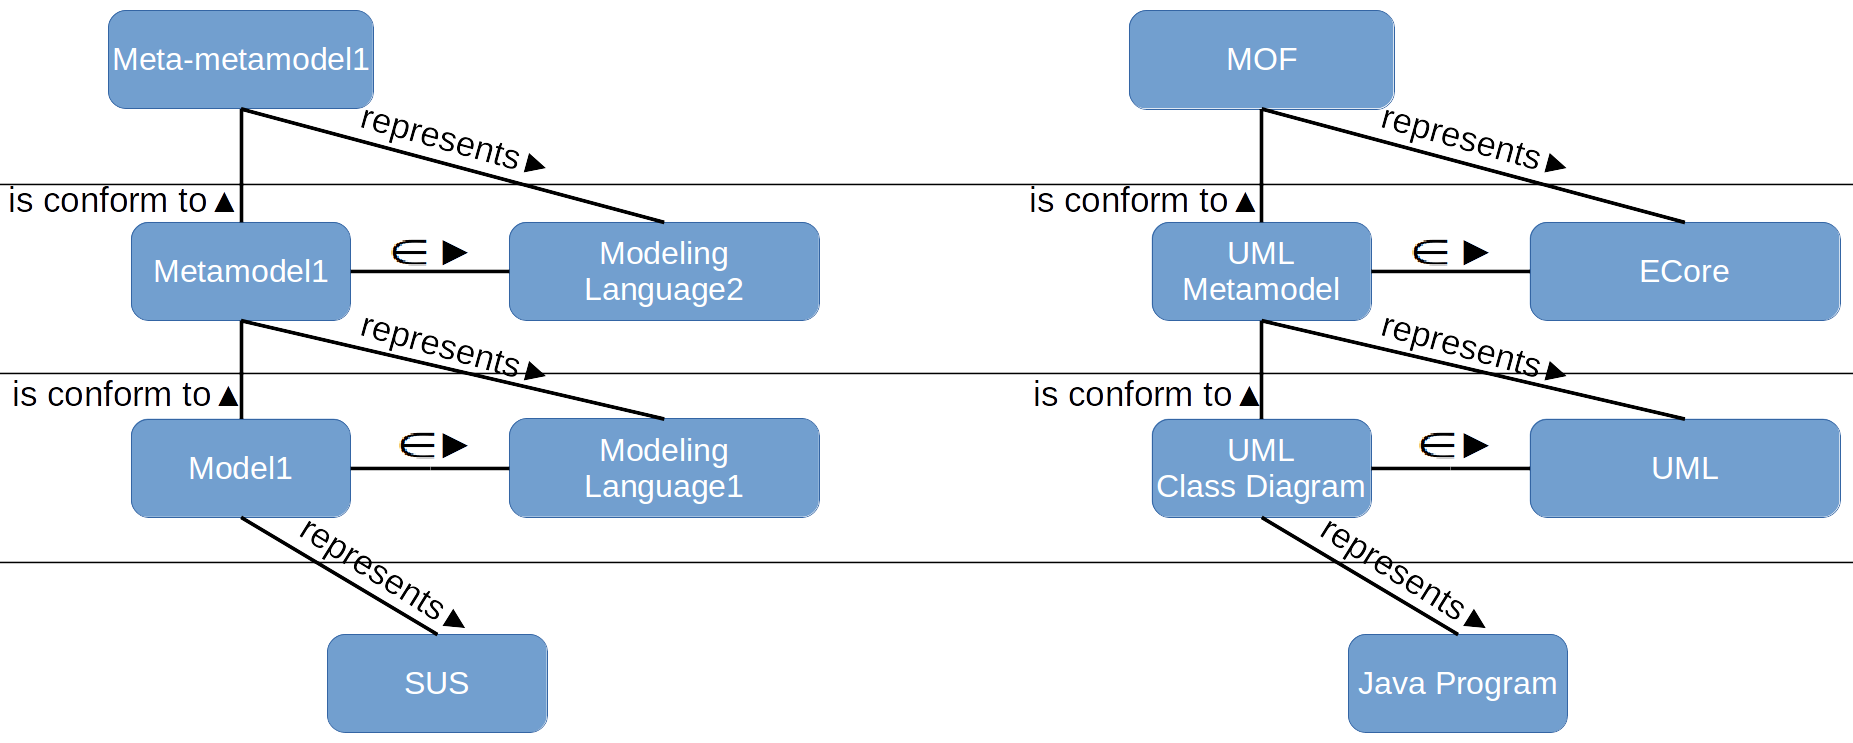
\includegraphics[width=\textwidth]{model_scheme}
		\end{subfigure}
		\begin{subfigure}[h]{.49\textwidth}
			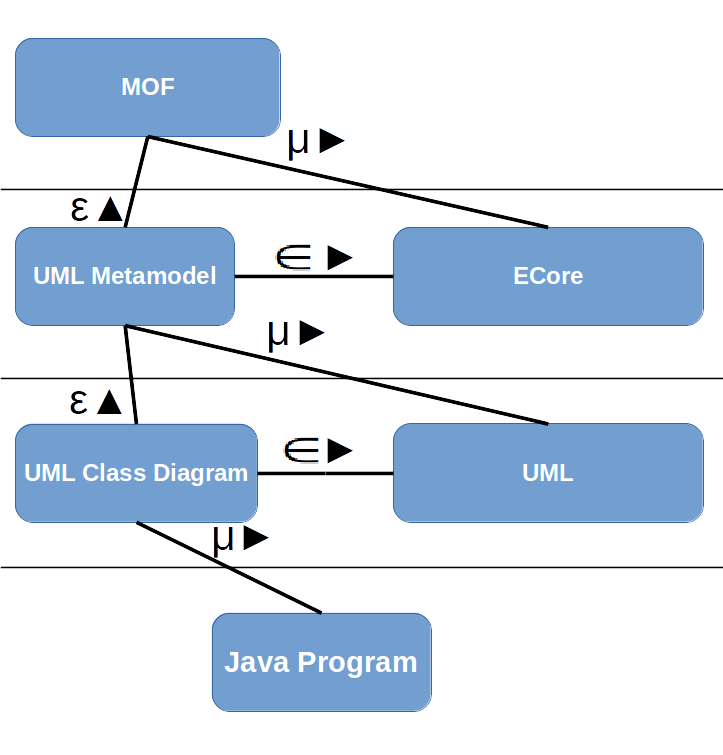
\includegraphics[width=\textwidth]{model_scheme_practice}
		\end{subfigure}
		\label{fig:model_scheme}
		\legend{Source: The author}
	\end{figure}
	
	\item[Model Relation:] Model relation here is defined abstractly as every relationship or constraint possible to happen between one source model and one target model. For instance, the models \emph{UML class diagram} and Java code have a relation, because once a new class is created in the class diagram, the correspondent class has to be created in the Java code. Moreover, a \emph{UML class diagram} with contracts definitions (pre and post-conditions) have a relation to the \emph{JUnit model}, once that the formers have to be tested correspondingly in the latter.

	%TODO: Note that? ok?
	\item[Model Transformation:] Model transformation can be viewed as common data transformation – very common in computer science – with the specificity of dealing with models \cite{czarnecki2006feature}. More specifically, model transformation is defined here as a function $t : M \rightarrow N$, where $t(m) = n$ means that a target model $n \in N$ is created from a source model $m \in M$, $M$ and $N$ being respectively the set of all valid models of the meta-models $\Phi_M$ and $\Phi_N$. Practical example: Creation of Java code from \emph{UML class diagram}. Note that, model transformation is by nature deterministic, unidirectional and does not preserve the information of the target model (e.g. comments in the Java code).

	%TODO: Note that? ok?
	\item[Model Synchronization:] The goal of model synchronization is to maintain all relations between the models of a system consistent/correct as updates are performed over them \cite{diskin2011model}. More specifically, model synchronization is defined here as a function $s : M \times M \times \Delta_M \times N \times N \times \Delta_M \rightarrow M \times N $, where $s(m_0,m_1,\delta_m,n_0,n_1,\delta_n) = (m_2,n_2)$ means that final synchronized models $m_2$ and $n_2$ are created from the initial synchronized models $m_0$ and $n_o$ and the modified non-synchronized models $m_1$ and $n_1$, considering the modifications (respectively $\delta_m$ and $\delta_n$) performed over both. Practical example: Modification of a method name ($\delta_m$) in the \emph{UML class diagram}($m_0$) has to be forwarded to the Java code($n_0$), without losing extra information of it (e.g. comments). Note that, model synchronization is deterministic, bidirectional and preserves the informations of the both models. Other terms for model synchronization are \emph{iterative} or \emph{information preserving bidirectional model transformation}.

	\item[Network of Models:] A network of models of a system $S$ is an undirected graph $G = (V,E)$, whereas each vertex $v_i \in V$ represents a unique model $i$ abstracting $S$, and an edge $(v_i, v_j)$ exists if, and only if there is a relation defined between both models $i$ and $j$. In the figure \ref{fig:network_example_01} is an example of a network of models, illustrating the possible complexity of such network. More discussion is to find in \citet{mens2006taxonomy}.

	\begin{figure}[h]
	    \caption{An example of a network of models very similar to the one developed in this work.}
	    \begin{center}
	        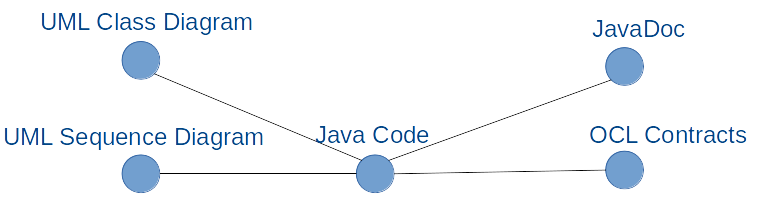
\includegraphics[width=25em]{network_example_01}   
	    \end{center}
	    \label{fig:network_example_01}
	    \legend{Source: The Author}
	\end{figure}

	\item[Meta Object Facility:] \emph{"The Meta Object Facility (MOF) provides an open and platform-independent metadata management framework and associated set of metadata services to enable the development and interoperability of model and metadata driven systems"} \citep{omg2015meta}. The MOF describes therefore the MOF modeling language, which is used to model the meta-metamodel utilized in this thesis. Essentially, it inherits much from the UML and deals with the ideas of classes, properties and associations, providing and extensible but simple fashion to define meta-models. The figure \ref{fig:emof_classes} shows the part of MOF.

	\begin{figure}[h]
	    \caption{Part of MOF definition, which handles basically classes, properties, operations, associations, and generalization.}
	    \begin{center}
	        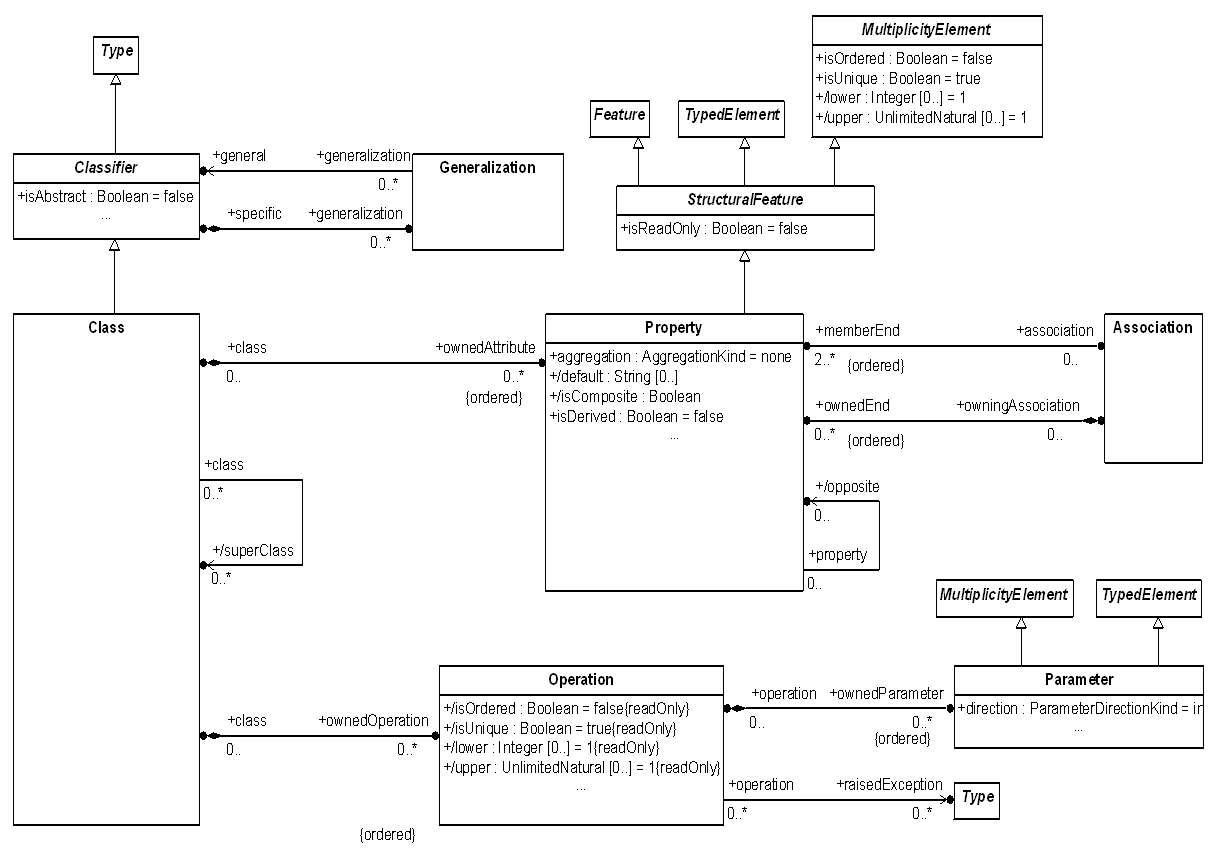
\includegraphics[width=35em]{emof_classes}   
	    \end{center}
	    \label{fig:emof_classes}
	    \legend{Source: \citep[p. 27]{omg2015meta}}
	\end{figure}

	\item[Ecore:] Ecore\footnote{https://eclipse.org/modeling/emf} is the meta-metamodel utilized in this thesis to describe all the applied meta-models (e.g the Java meta-model). Ecore is an initiative of the EMF Project and aims to provide not only a meta-metamodel but a set of tools for criating meta-models, like an Eclipse plug-in generation feature, that enables the model developer to easily test and debug its meta-models. The Ecore meta-metamodel is at least similar to the essential MOF standard, and that is the reasons it is applied here. A proof of such compliance is not know by us though. The figure \ref{fig:ecore_relations} shows the essential part of Ecore.

	\begin{figure}[h]
	    \caption{Ecore definition illustrating the use of classes, attributes, operations, references and super types, analogously to the figure \ref{fig:emof_classes}}
	    \begin{center}
	        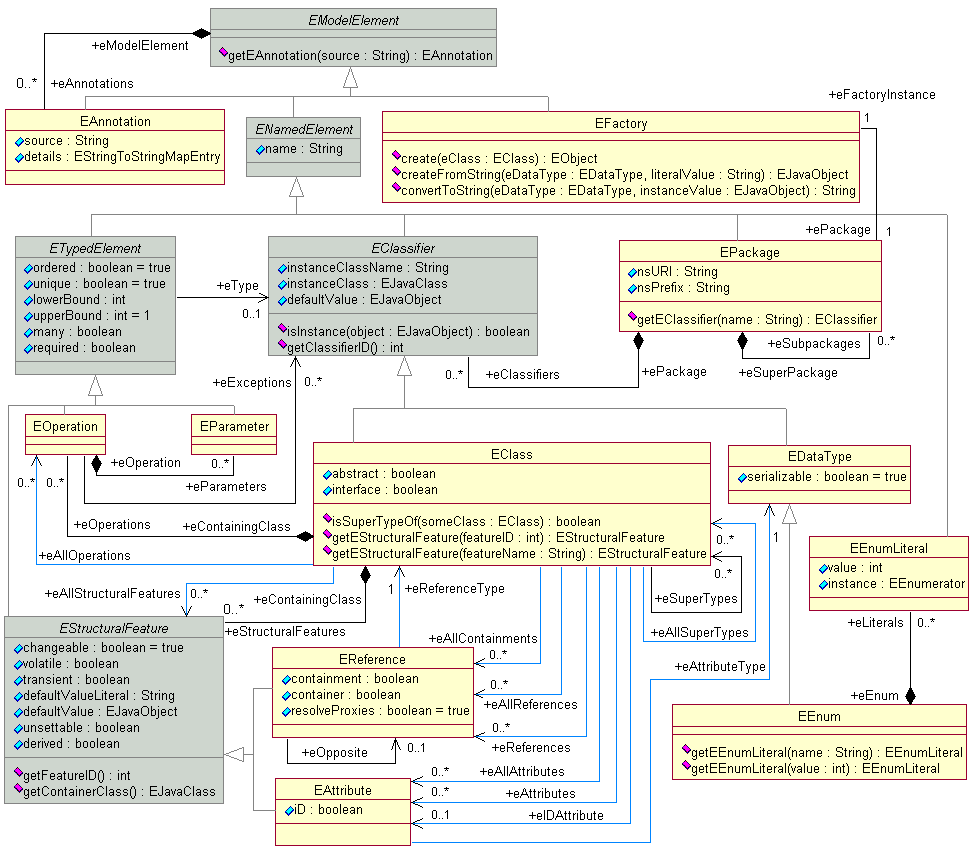
\includegraphics[width=35em]{ecore_relations}   
	    \end{center}
	    \label{fig:ecore_relations}
	    \legend{Source: http://download.eclipse.org/modeling/emf/emf/javadoc/2.9.0/org/eclipse/emf/ecore/package-summary.html. On the December 29th, 2015}
	\end{figure}

	\item[Triple Graph:] With the use of a triple graph a relation between a source model S and a target model T are abstracted into a triple $(G_s,G_c,G_t)$ – where $G_s$ is the graph representation of source model elements, $G_t$ is the graph representation of target model elements, and $G_c$ represents the correspondence between the two set of model elements – together with two mappings $s_g: G_c \rightarrow G_s$ and $t_g: G_c \rightarrow G_t$, which bind the three graphs \citep{hermann2011correctness}.
	
	In this case, an addition in the triple graph $G = (G_s,G_c,G_t)$, that leads to a new triple graph $H = (H_s,H_c,H_t)$ consists in a triple graph morphism $m: G \rightarrow H$, with $m = (m_s,m_c,m_t)$. According to the figure \ref{fig:tg_morphism}.

	\begin{figure}[h]
	    \caption{The morphism $m: G \rightarrow H$ is a triple graph $m = (m_s,m_c,m_t)$.}
	    \begin{center}
	        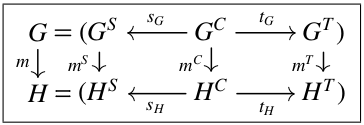
\includegraphics[width=20em]{tg_morphism}   
	    \end{center}
	    \label{fig:tg_morphism}
	    \legend{Source: \citep{hermann2011correctness}}
	\end{figure}

	\item[Triple Rule:] A triple rule is a triple graph morphism $t_r = (s, c, t) : L \rightarrow R$, where $L$ and $R$ are called respectively the left-hand the right-hand sides (resp. LHS and RHS) \citep{ehrig2007information}.
	
	\item[Triple Axiom:] A triple axiom is a triple rule $t_a = (s, c, t) : \emptyset \rightarrow R$. In order to apply such definitions in the practice, it is common to use attributed graphs and a easier to read diagram scheme depicted in the figure \ref{fig:tgg_axiom_rule}.


	\begin{figure}[h]
	    \caption{In this kind of diagram for triple rules a triple graph is represented by three columns (left model domain, correspondence domain, and right model domain) each one representing respectively the source model elements, the correspondence between source and target and finally the target model elements. A triple rule in turn is represented by a triple graph in black (left-hand side) plus a triple graph in green (right-hand side) (see \ref{fig:tgg_rule}). Because an axiom is a triple rule with empty left-hand side, only green graph occurs in an axiom (see \ref{fig:tgg_axiom}).}
	    \label{fig:tgg_axiom_rule}
	    \begin{subfigure}{\textwidth}
		    \caption{Triple axiom example for the relation between UML and Java}
	        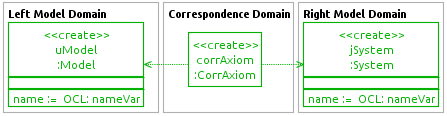
\includegraphics[width=\textwidth]{tgg_axiom} 
	        \label{fig:tgg_axiom}  
	    \end{subfigure}
	    \begin{subfigure}{\textwidth}
		    \caption{Triple Rule example for the relation between UML package and Java package}
	        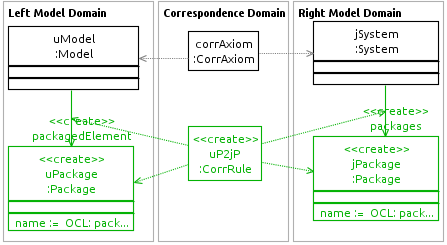
\includegraphics[width=\textwidth]{tgg_rule} 
	        \label{fig:tgg_rule}  
	    \end{subfigure}
	    \legend{Source: The author}
	\end{figure}

	\item[Triple Graph Grammar:] A triple graph grammar $TGG = (t_a, T_{rules}) $ consists of a triple axiom $t_a$ and a set of triple rules $T_{rules}$ \citep[p. 4]{giese2010toward}. While one triple graph can be used as a description of a relation between two meta-models, one TGG describes the language of the these two related models and serves rather as description of consistency. Nevertheless, extra rules can be derived from a TGG, in order to create the operational semantic of a transformation procedure \citep{giese2010toward}. Figure \ref{fig:transformation_scheme} summarizes the so far defined terms.

	\begin{figure}[h]
	    \caption{Illustration of the definitions of model relation, transformation and synchronization as well as triple graph grammars (TGG). Relations between metamodels are coded by triple graphs; additions in the models are coded by triple rules, which are then organized in a TGG. A TGG can be used to derive operational semantic definitions. The concept of modeling language is pictured as red lines.}
	    \begin{center}
	        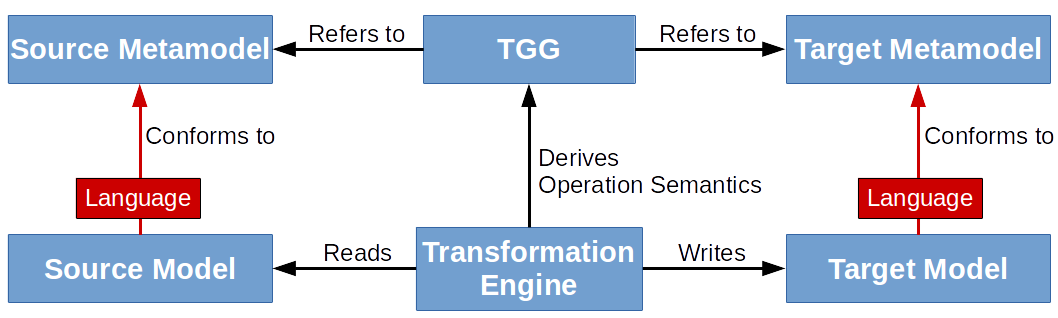
\includegraphics[width=25em]{transformation_scheme}
	    \end{center}
	    \label{fig:transformation_scheme}
	    \legend{Source: Adapted from \citet[p. 623]{czarnecki2006feature}}
	\end{figure}
\end{description}

%---------------------------------------------
% Section
%---------------------------------------------
\chapter{State of the art}
%TODO: us?
Some endeavors have been made in order to code relations between some meta-models and mainly to develop theoretical results and synchronization methods. \citeauthor{heidenreich2010closing} present in \citeyearpar{heidenreich2009jamopp} and \citeyearpar{heidenreich2010closing} a Java meta-model using \emph{Ecore}, what influenced considerably the development of our work, although it has not been used by us because of its size and unnecessary comprehensiveness for our needs. \citet{greenyer2008tggs} comes up with a transformation between \emph{UML activity diagrams} and \emph{CSP diagrams} using \emph{TGG}. \citet{foss2011uml} defined the translation between \emph{UML} and \emph{Simulink} using graph grammars. \citet{blouin2014synchronization} reports about the synchronization between some specific meta-models of the automotive standards and influences our work, by using the same modeling language and transformation method as us, namely \emph{EMF} \citep{steinberg2008emf} and \emph{MoTE} \citep{giese2010toward}. Finally \citet{giese2010model} introduce their approach to the synchronization of two automotive industry meta-models, lightening in the paper the \emph{MoTE} tool and its algorithm for synchronization.

We judge that the \emph{MoTE} transformation tool is the most adequate option for our needs, once literature about it is widely available (see also \citep{giese2009efficient} and \citep{hildebrandt2012mdelab}). Nevertheless there are other attempts to build a model synchronization tool, like the \emph{ATL Eclipse Plug-in} \citep{jouault2008atl}, which uses the \emph{Atlas Transformation Language} to code the relations between models; the Medini QVT \footnote{http://projects.ikv.de/qvt}, which claims to implement the \emph{Query/View/Transformation Language} to code the relations; and the FUJABA \citep{nickel2000fujaba}, in which relations are coded using \emph{Triple Graph Grammars}. \citet{hildebrandt2013survey} also publicized a survey on synchronization tools based on TGG. Other publications aim to solve specific problems, like the ones in \citet{hermann2011correctness}, \citet{xiong2007towards}, \citet{giese2006incremental}, \citet{ivkovic2004tracing}, or \citet{song2011instant}, where advanced algorithms for bidirectional synchronization have been proposed.

A research road-map for model synchronization found in \citet{france2007model} gives an overview on the realm, and together with \citet{mattsson2009linking} show an interesting point of view about the challenges. \citet{seidewitz2003models} writes an interesting reflection  about what models mean and how to interpret them and in \citet{mens2006taxonomy} a taxonomy for model transformation is proposed, what helps to carry more precise analysis. In \citet{czarnecki2006feature} a survey was driven and a framework for classification of model transformation approaches was presented. In \citeauthor{diskin2014towards} \citeyearpar{diskin2014towards} and \citeyearpar{diskin2016three} a taxonomy for a network of models is presented and in \citet{diskin2011model} a theoretical algebraic basis is proposed.

Additionally, one can judge by the date of publication of these works, that the topic of model synchronization is extremely active and is actually the edge of current academic research, what motivates even more the development of this thesis.

%%%%%%%%%%%%%%%%%%%%%%%%%%%%%%%%%%%%%%%%%%%%%%%%%%%%%%%%%%%%%%%%%%%%%%%%
% Chapter
%%%%%%%%%%%%%%%%%%%%%%%%%%%%%%%%%%%%%%%%%%%%%%%%%%%%%%%%%%%%%%%%%%%%%%%%
\chapter{Meta-model Relations in the Java Technological Space}
\label{chapter:metamodel_relations}
With the terms and the theoretical basis clarified, the report of the main development phase of the thesis is shown below. The idea here is first to present the selected network of meta-models, by describing what each model represents and how they relate to each other. Then the developed meta-model definitions and the relations between them are exposed, as well as the justification of the choices made during the work.

%---------------------------------------------
% Section
%---------------------------------------------
\section{The Network of Meta-models}
The choice of which models are used in a certain Java program may vary considerably depending on the context of the development and the software requirements, which themselves can range from high dependability (e.g. airplane software) to continuous evolution (e.g. applications for cellphones), for example. Nevertheless, we selected a few typical models and the relations between them and created a network of meta-models. The figure \ref{fig:network_metamodels} depicts this network. The bold printed vertices and edges represent respectively the meta-models and the relations, that are treated more deeply in this thesis, namely \emph{Java}, \emph{UMLClassDiagram}, \emph{UMLSequenceDiagram}, \emph{UMLContract} and \emph{UnitTest}, whereas the other vertices are by virtue of the scope of this thesis some rather more briefly discussed meta-models, namely \emph{UMLUseCaseDiagram}, \emph{RequirementDiagram}, \emph{JavaDoc}, \emph{UMLStateMachine}, \emph{ERDiagram}, \emph{FormalSpecification}. This does not mean however, that they are not worth further studying.

\begin{figure}[h]
    \caption{A network of meta-models in the Java technological spaces}
    \begin{center}
        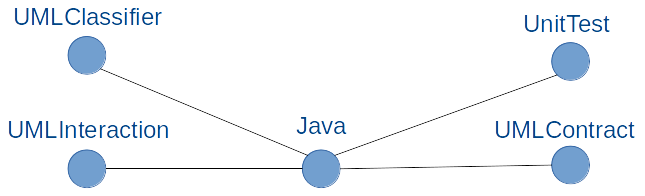
\includegraphics[width=30em]{network_metamodels}
    \end{center}
    \label{fig:network_metamodels}
    \legend{Source: The author}
\end{figure}

The central element of the network is the \emph{Java} meta-model. A Java model (or, Java code) contains both structural and behavioral information about the system, which is represented among other elements through \emph{classes}, \emph{fields}, \emph{methods} and \emph{statements}.

%TODO: Imperative ok?
Once a meta-model might be relatively big and comprise a huge number of elements, it is interesting to split it into smaller pieces for a specific set of relations. Take for example the UML, that includes a large number of different concerns (e.g. classifiers, state machines, activities, interaction, etc) and may be split into sub meta-models in order to ease the writing of the relations. For this reason we separate the UML into \emph{UMLClassDiagram}, \emph{UMLSequenceDiagram}, \emph{UMLContract}, \emph{UMLUseCaseDiagram} and \emph{UMLStateMachineDiagram}. The first is constructed around the concepts of \emph{class}, \emph{property}, \emph{operation}, \emph{interface} and \emph{package}. This meta-model is usually used to describe the structure of a object oriented Java program through a class diagram, representing the definition of its classes, field and methods, but leaving out behavioral aspects. The relations between \emph{UMLClassDiagram} and \emph{Java} is then given by an almost direct translation between their elements. A \emph{class} in the former is transformed into a \emph{class} in the latter, a \emph{property} in a \emph{field}, an \emph{operation} in a \emph{method} and so on.

To represent some behavioral aspects, \emph{UMLSequenceDiagram} is used instead. The elements of this meta-model are usually reproduced with sequence diagrams, where \emph{lifelines} and \emph{messages} provide information about the sequence of event occurrences. In a Java program it may correspond to the sequence of calls inside a specific method. This means, the semantical information of each sequence diagram could be brought to the correspondent method in the Java model.

\emph{UMLContract} is based on the ideas of design-by-contract, whose main goal is to improve reliability of object oriented software \citep{meyer1992applying}, and where operations have \emph{pre} and \emph{postconditions} as well as \emph{invariants}. Its relation with \emph{Java} is basically, that each constraint of the contracts can (1) be tested as assertions and (2) expressed in terms of annotations in the Java source-code. Moreover, one can have check methods in Java, which serve to verify the constraints of the class and therefore are supposed to be updated as soon as the contracts undergo changes. Related to contracts are also \emph{Formal Specifications}, these taking several different forms, among them the Z Notation (see \citep{spivey1992z}), which itself also refers to \emph{pre} and \emph{postconditions}.

The \emph{UnitTest} endeavors to enhance the software quality by means of tests. It tests small units of code, by basically verifying the pre and postconditions as well as invariants of each method. Because unit tests for Java programs are usually written in Java, we use the same meta-model for the vertices \emph{Java} and \emph{UnitTests} of our network. Anyways, the relation between both is based on creating test cases in the latter according to the contract annotations (e.g pre and postconditions, invariants, examples, etc) present in the methods of the former.

Moreover, \emph{UML Use Cases Diagrams} are used to relate \emph{Actors} (basically users of the program) and \emph{Use Cases} (specifications of behavior), and therefore have a relationship with \emph{Requirement Diagrams}, a very common tool on information system analysis for description of features of a system, and with \emph{Sequence Diagrams} (discussed before) and \emph{State Machine Diagrams}, two artifacts aiming to describe the behaviors specified by the use cases \citep[p. 637]{omg2007unified}. \emph{State Machines} are well known means for modeling functionalities of Java programs, rely on \emph{states} and \emph{transitions} and relates to \emph{Use Cases Diagrams} in the sense that it describes the behavior of a \emph{Use Case}. For this reason, one may argue, that the behavior expressed by \emph{State Machines} may also be synchronized with the implementaion of methods in the \emph{Java source-code}.

The linking from \emph{Requirement Diagrams} to \emph{Unit Tests} has been proposed by \citet{noack2013automatic} and by \citet{post2009linking} and a kind of linking to source-code has been proposed by \citet{antoniol2002recovering}. \emph{JavaDoc} models play an important role as well, as they serve as program documentation for the developers. A transformation from the Java source-code to a \emph{JavaDoc} model is already achievable through the \emph{JavaDoc Tool} \footnote{http://www.oracle.com/technetwork/articles/java/index-jsp-135444.html}, which transforms comments from the source-code into HTML documentation.

Finally, there is the \emph{ERDiagram} (Entity-relationship model, see \citep{chen1976entity}), used to construct data models and is applied specially to describe database schemes through basically \emph{Entities}, that often correspond to \emph{Java classes}, and \emph{Relationships} between them, what may be seen often as \emph{Java attributes}.

%---------------------------------------------
% Section
%---------------------------------------------
\section{Meta-model Definitions}
As stated in the last section, the meta-models highlighted in the figure \ref{fig:network_metamodels} have its meta-models defined here, and the relation between them formalized. The meta-models \emph{UMLClassDiagram}, \emph{UMLSequenceDiagram}, \emph{UMLContract}, and \emph{Java} $-$ which serves also for the vertice \emph{UnitTest} $-$ are explained below with help of a running example.

The modeling language used to write these meta-models is the \emph{EMF Ecore} and the tool used is the special version for model development of the \emph{Eclipse Mars 4.5.1 IDE\footnote{https://projects.eclipse.org/releases/mars}}, which eases the creations of models and their diagrams as well as the generation of plug-ins necessary for running the transformations. For this reason \emph{Eclipse IDE} seems to be more suitable than the alternatives \emph{Netbeans IDE}\footnote{https://netbeans.org} or FUJABA \citep{nickel2000fujaba}, whose support or popularity in the community are not so valuable. The \emph{EMF Ecore} language has been chosen not only for its extensible documentation and popularity in the community, but also for its ease to use in the \emph{Eclipse IDE}. The meta-models are listed in the sections below.

%-------------------
% Subsection
%-------------------
\subsection{UML Class Diagram}
%TODO: First person again
%TODO: Update with new concerns of the uml
The meta-model utilized for \emph{UMLClassDiagram} (also for \emph{UMLSequenceDiagram}, \emph{UMLContract}) represents the version 2.0 of the UML standard and is provided by the \emph{EMF plug-in}\footnote{https://eclipse.org/modeling/emf} for Eclipse, which clearly integrates easily with the IDE and seems to be suitable for our needs. Alternatively we could use the meta-model provided by the OMG, but then unnecessary work of adaption could late our progress. The figure \ref{fig:uml_metamodel_class} addresses a simplified view of the \emph{UMLClassDiagram}. Elements in blue are \emph{EMF Ecore} abstract elements, whilst elements in yellow are concrete. Some features like operations and some relations between elements were omitted for a better visualization. 

\begin{figure}[h]
    \caption{Simplification of the \emph{UMLClassDiagram} meta-model}
    \begin{center}
        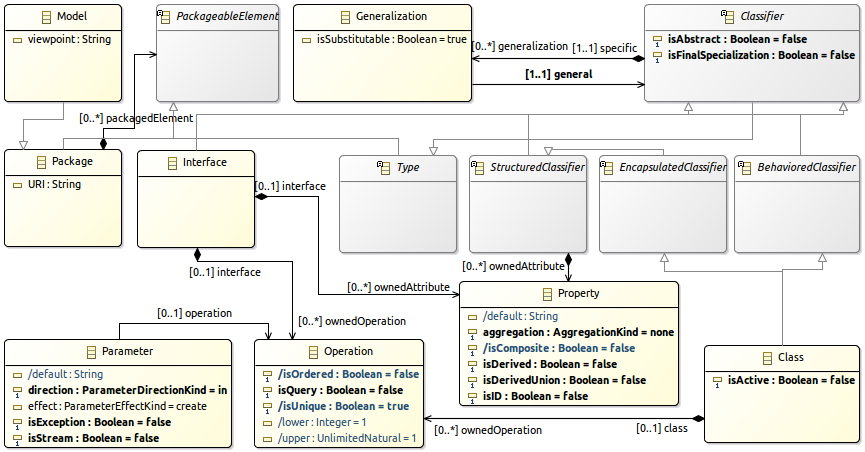
\includegraphics[width=35em]{umlClassDiagramSimple01}
    \end{center}
    \label{fig:uml_metamodel_class}
    \legend{Source: Image created by the author using the \emph{Eclipse IDE}. Meta-model from \emph{EMF plug-in}}
\end{figure}

The \emph{Model} (top, link on figure \ref{fig:uml_metamodel_class}) represents the whole model and is the root element of a class diagram, in the sense every other element is contained by it. \emph{Model} inherits \emph{Package}, and thus may contain \emph{Packageable Elements}. Because \emph{Packages} inherit \emph{Packageable Elements}, they may be contained by the \emph{Model}, what is the most common case. An example of a \emph{UMLClassDiagram} model (not the meta-model) is depicted in the figure \ref{fig:uml_metamodel_class_example} in two forms: In abstract and in concrete syntax. There a \emph{Model} named \emph{Example01} contains a \emph{Package} named \emph{main}.

A \emph{Package} may contain according to these scheme other \emph{Packages} as well as a \emph{Classifier} (center on the figure \ref{fig:uml_metamodel_class}), because this one inherits \emph{Packageable Element}.The two classifiers handled in the figure are \emph{Class} and \emph{Interface}. The model if the running example contains the \emph{Classes} \emph{Person}, \emph{Driver}, and \emph{Car}; and the \emph{Interface} \emph{Drivable}.

%TODO: write about Parameter

\begin{figure}[h]
    \caption{An example of a model \emph{UMLClassDiagram} visualized in two different ways, containing one \emph{Model} (\emph{Example01}), one \emph{Package} (\emph{main}), three \emph{Classes} (\emph{Person}, \emph{Drive} and \emph{Car}), and one \emph{Interface}, namely \emph{Drivable}.}
    \centering
	\begin{subfigure}[h]{.35\textwidth}
		\caption{Abstract Syntax}
		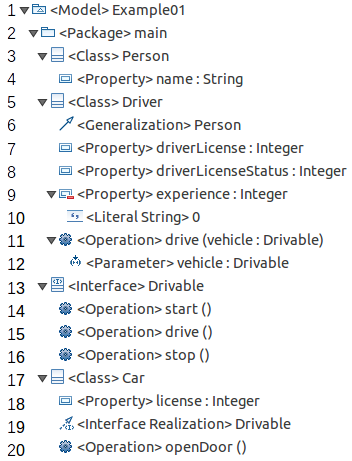
\includegraphics[width=\textwidth]{umlClassDiagramExample01}
	\end{subfigure}
	\begin{subfigure}[h]{.64\textwidth}
		\caption{Concrete Syntax}
		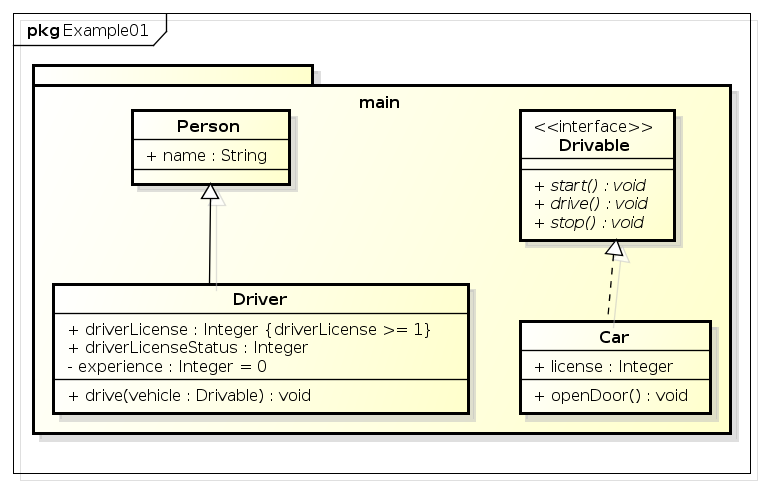
\includegraphics[width=\textwidth]{umlClassDiagramExample01_Diagram}
	\end{subfigure}
    \label{fig:uml_metamodel_class_example}
    \legend{Source: Image created by the author using the \emph{Astah Software}\footnote{http://astah.net}.}
\end{figure}

According to the meta-model, a \emph{Classifier} may have a \emph{Generalization} (i.e. inheritance), illustrated with a straight arrow from \emph{Driver} to \emph{Person} in the example on the figure \ref{fig:uml_metamodel_class_example}, or an \emph{InterfaceRealization}  illustrated with a dashed arrow from \emph{Car} to \emph{Drivable}. Moreover, a \emph{Class} is possible to have not only \emph{Properties} (through the aggregation \emph{ownedAttribute}), but also \emph{Operations} (through the \emph{ownedOperation} attribute). This characteristic is analogous to \emph{Interfaces}. In the running example the \emph{Person} has the \emph{Property name}, as well as the \emph{Driver} has the \emph{Property driverLicense} and the \emph{Operation drive(Drivable):void}. 

%-------------------
% Subsection
%-------------------
\subsection{UML Sequence Diagram}
The \emph{UMLSequenceDiagram} is essentially based on the elements \emph{Interaction}, \emph{Lifeline}, and \emph{Messages}. A simplified view of the meta-model is given on the figure \ref{fig:uml_metamodel_sequence}. According to \citet[p. 563]{omg2007unified}: \emph{"Interactions [...] are used to get a better grip of an interaction situation"} \citep[p. 563]{omg2007unified}, by being so the important aspect of \emph{Sequence Diagram} are the exchange of messages between object (i.e. interaction). Sequence diagrams are quite flexible in regard to its semantics, so developers interpret the exchange of messages in different ways. Nevertheless, they are interpreted in this thesis in a rather simpler manner. An \emph{Interaction} models one scenario, in which an \emph{Operation} of a \emph{Class} is executed, and contains one or more \emph{Lifelines}, that express the life of an instance of a class. A concrete illustration of these elements is to find in the example in the figure \ref{fig:uml_metamodel_sequence_example_diagram}.

\begin{figure}[h]
    \caption{Simplification of the \emph{UMLSequenceDiagram} meta-model}
    \begin{center}
        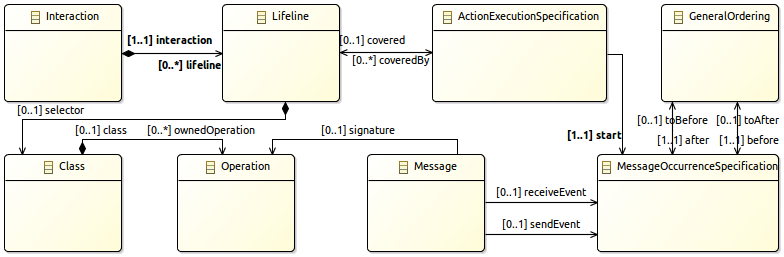
\includegraphics[width=\textwidth]{umlSequenceDiagramSimple01}
    \end{center}
    \label{fig:uml_metamodel_sequence}
    \legend{Source: Image created by the author using the \emph{Eclipse IDE}. Meta-model from \emph{EMF plug-in}}
\end{figure}

One \emph{Lifeline} is connected to a \emph{Class} through the attribute \emph{selector} and is \emph{covered by} one \emph{Action Execution Specification}, which in a sequence diagram is depicted by a rectangle over the \emph{Lifeline} and symbolize the time, during which the respective class is executed. An \emph{Action Execution Specification} has then a \emph{MessageOccurenceSpecification} as \emph{start} point, which itself is related to a \emph{Message}. Finally, each \emph{Message} is linked to two \emph{MessageOccurenceSpecifications} $-$ one \emph{receiveEvent} that lies on the beginning and one \emph{sendEvent} that lies on the end of the \emph{Message}); and has a \emph{signature} of an \emph{Operation}. The comprehension of this interpretation over \emph{Sequence Diagrams} requires the reader to grasp the figure \ref{fig:uml_metamodel_sequence_example}

\begin{figure}[h]
    \caption{An example of a model \emph{UMLSequenceDiagram} containing one \emph{Interaction} (\emph{Interaction01}), two \emph{Lifelines} (\emph{:Driver} and \emph{:Drivable}), and four \emph{Messages}.}
    \centering
   	\begin{subfigure}[h]{\textwidth}
   		\caption{Abstract Syntax}
   		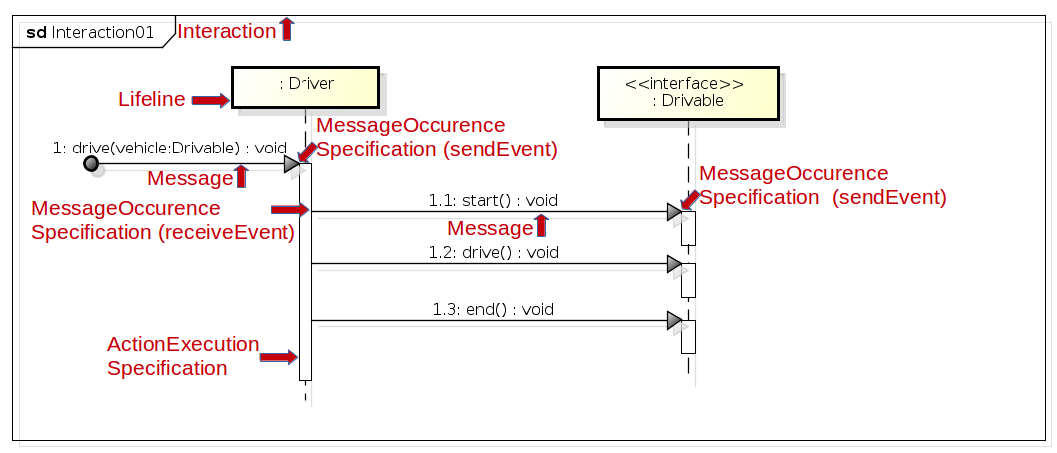
\includegraphics[width=\textwidth]{umlSequenceDiagramExample01}
   	\end{subfigure}
   	\begin{subfigure}[h]{\textwidth}
   		\caption{Concrete Syntax}
   		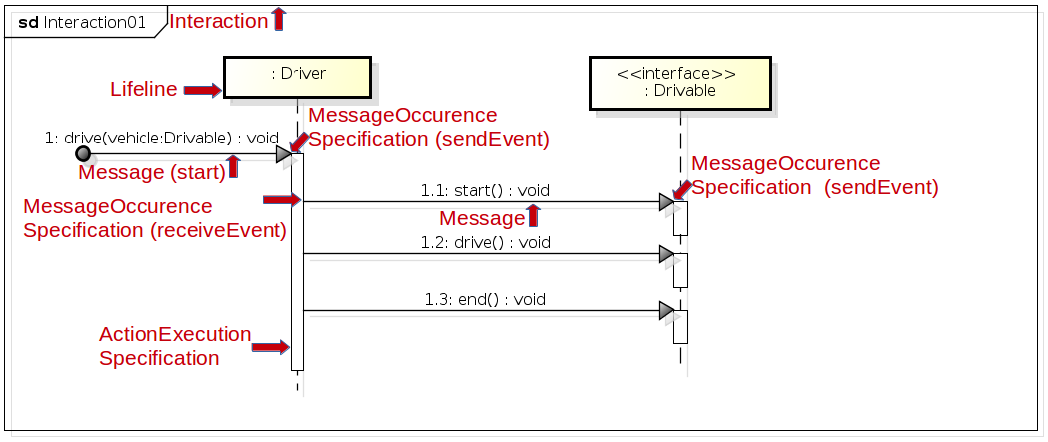
\includegraphics[width=\textwidth]{umlSequenceDiagramExample01_Diagram}
   		\label{fig:uml_metamodel_sequence_example_diagram}
   	\end{subfigure}
    \label{fig:uml_metamodel_sequence_example}
    \legend{Source: Image created by the author using the \emph{Astah Software}\footnote{http://astah.net}.}
\end{figure}

To model the order in which the \emph{Messages} occur, a \emph{GeneralOrdering} establishes an order between two \emph{MessageOccurenceSpecifications}, by signalizing which of them occur \emph{before} or \emph{after} the other. So in the running example there is a \emph{GeneralOdering} instance holding the \emph{MessageOccurenceSpecifications} related to the \emph{Message 1} as happening \emph{before} the one related to the \emph{Message 1.1} (that is held as \emph{after}).

As stated before, developers tend to interpret and utilize sequence diagrams in different fashions. For this thesis a set of assumptions is made in regard to that, among them lifelines represent only classes (excluding thus representation of actors); and only synchronous message are handled.

%-------------------
% Subsection
%-------------------
\subsection{UML Contract}
The \emph{UMLContract} is a slice of the \emph{UML} meta-model, that aims basically to provide constraints to \emph{Operations} and \emph{Properties} of \emph{Classes}. \emph{Operations} may have \emph{pre}, \emph{postconditions}, as well as \emph{Invariants}, which are modeled through the EMF class \emph{Constraint} (on the top of the figure \ref{fig:uml_metamodel_contracts}).

\begin{figure}[h]
    \caption{Simplification of the \emph{UMLContract} meta-model}
    \begin{center}
        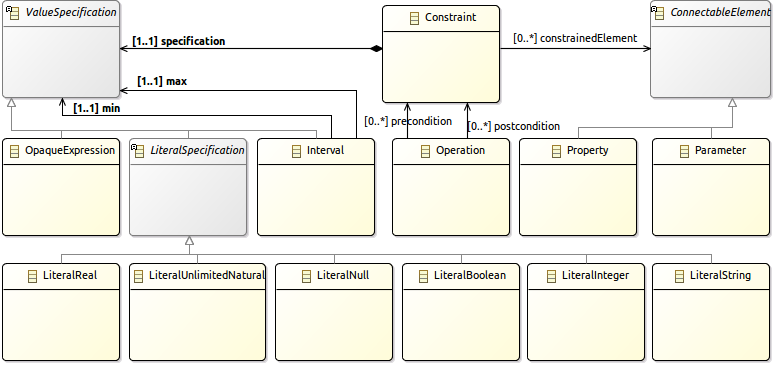
\includegraphics[width=\textwidth]{umlContractSimple01}
    \end{center}
    \label{fig:uml_metamodel_contracts}
    \legend{Source: Image created by the author using the \emph{Eclipse IDE}. Meta-model from \emph{EMF plug-in}}
\end{figure}

A \emph{Constraint} may have then \emph{constrainedElements}, which in the scope of this thesis are whether \emph{Properties} or \emph{Parameters} (of operations). In addition, it has also a \emph{ValueSpecification}, defining the constraint itself, that in this thesis may be a \emph{OpaqueExpression} or a \emph{Interval}. The former is rather a free definition of the constraint composed by a String \emph{body}, and the \emph{language}, in which it is written (see lines 16 to 19 in figure \ref{fig:uml_metamodel_contracts_example}). The latter defines a interval of values, in which the \emph{constrained element} has to lie. Therefore it has one \emph{value specification} for the minimal and one for the maximal value. Here only \emph{intervals} with one \emph{literal integer value specification} for the minimal value will be handled, see an example in the lines 6 to 7 in figure \ref{fig:uml_metamodel_contracts_example}.

\begin{figure}[h]
    \caption{The expanded version of the model from the picture \ref{fig:uml_metamodel_class_example} including elements from \emph{UMLContract}, namely lines 6 to 7 and 14 to 15 (\emph{Constraint} with \emph{Interval}), and lines 16 to 19 (\emph{Constraint} with \emph{OpaqueExpression}). Only abstract syntax is used for this example.}
    \begin{center}
        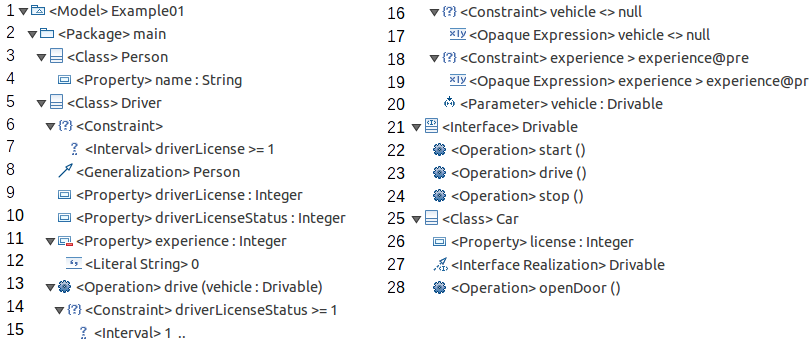
\includegraphics[width=28em]{umlContractDiagramExample01}
    \end{center}
    \label{fig:uml_metamodel_contracts_example}
    \legend{Source: Image created by the author using the \emph{Eclipse IDE}.}
\end{figure}

%-------------------
% Subsection
%-------------------
\subsection{Java}
A \emph{Java} model is usually the main artifact of a network of models, in that it comprises much information (both structural and behavioral) about the system under study. It can be visualized either as the digram in the figure \ref{fig:java_metamodel_example} or as plain-text (figure \ref{fig:java_metamodel_example_text01}). The first option is used here, since it seems to be more suitable when handling the model for synchronization than a plain-text source-code format. Nevertheless, there are techniques\footnote{https://eclipse.org/modeling/m2t} to transform one format into another.

A new meta-model for \emph{Java} was designed in regard to the necessities of this work and includes not only structural elements (e.g. \emph{Packages}, \emph{Classes}, \emph{Fields}, etc.), but also some behavioral aspects (e.g. \emph{Statements}), the latter are very shallowly modeled here, but could be further developed in future works. Other possibilities for the meta-model included the meta-model\footnote{http://www.eclipse.org/modeling/emf/downloads} provided by the \emph{Eclipse IDE}, whose simplicity hindered its use; or yet the one found in \citet{heidenreich2010closing}, but this one happens to be so extensive that could bring unnecessary complexity to this thesis. The figure \ref{fig:java_metamodel} reports the complete \emph{Java} meta-model created. Elements in blue are \emph{EMF Ecore} abstract elements, whilst elements in yellow are concrete.

\begin{figure}[h]
    \caption{The Java meta-model created. It goes beyond the common classes and attributes scenario, by comprising also annotations and statements.}
    \begin{center}
        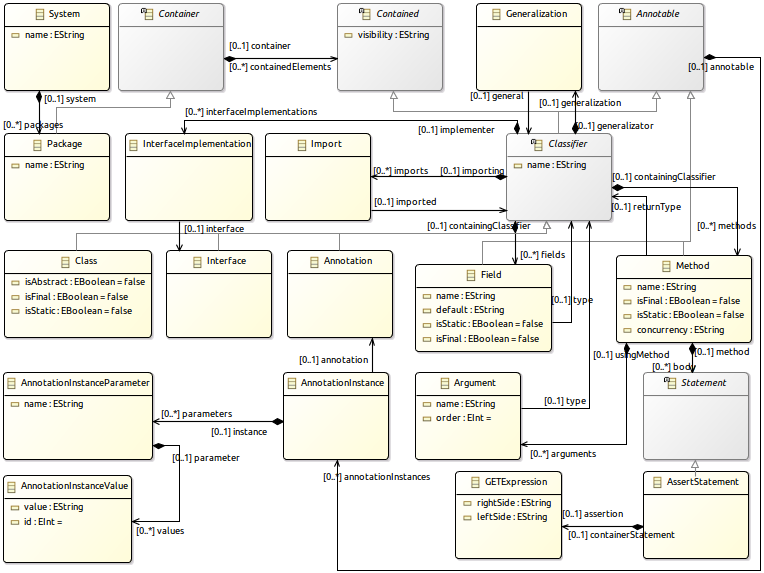
\includegraphics[width=\textwidth]{javaMetamodel}
    \end{center}
    \label{fig:java_metamodel}
    \legend{Source: Image created by the author using the \emph{Eclipse IDE}.}
\end{figure}

The root element is the \emph{System} (on the left top of figure \ref{fig:java_metamodel}) and represents the whole Java program. It contains \emph{Packages}, that, because of the \emph{Container} inheritance, contains \emph{Classifiers} (through the \emph{Contained} inheritance). The example on the picture \ref{fig:java_metamodel_example} illustrates concrete types of \emph{Classifiers} in the lines 3, 5 and 48 (\emph{Class}) and 44 (\emph{Interface}).

One \emph{Classifier} may contain \emph{Fields} (lines 4, 6, 10, 11, 49), \emph{Methods} (lines 12, 28, 31, 33, 35, 37), \emph{Imports} (lines 40 to 43), in addition to \emph{interface implementations} (line 54), that refer to one \emph{Interface}; and to one \emph{Generalization} (line 39), also known as inheritance or extension, which refers to another \emph{Classifier} as its \emph{general}.

A \emph{Method} may have zero or more \emph{Arguments}, also known as parameters; likewise \emph{Statements} (to find on the left bottom of the picture \ref{fig:java_metamodel}). In this imperative perspective of the \emph{Java} meta-model, each method has thus an ordered list of \emph{Statements}, representing usually commands that carve the behavior of the program. In a full representation of the \emph{Java} meta-model, they could be of several kinds (e.g. arithmetic expression, logic expression, method call, control structure like \emph{if}), but for the scope of this bachelor thesis only \emph{assert statements} are modeled. An \emph{AssertStatement} basically tests a logical expression. If it does not hold, than an exception is thrown. The only logical expression supported here is the \emph{greater-or-equal expression} (\emph{GETExpression}, left bottom on the picture \ref{fig:java_metamodel}), but again the construction of a more complete meta-model shall be possible in a wider scope. An example of a \emph{Method} with \emph{AssertStatement} is to find on the lines 28 to 30 and 33 to 36 of the picture \ref{fig:java_metamodel_example}.

\begin{figure}[h]
    \caption{The equivalent \emph{Java} version of the \emph{UML} models from the pictures \ref{fig:uml_metamodel_class_example},  \ref{fig:uml_metamodel_contracts_example} and \ref{fig:uml_metamodel_sequence_example} in abstract syntax.}
    \begin{center}
        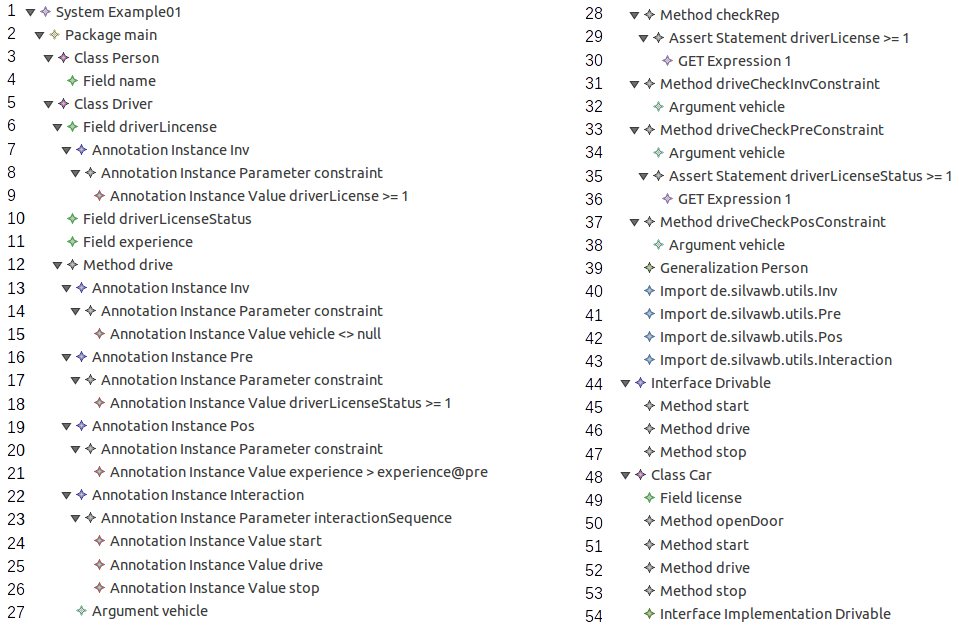
\includegraphics[width=38em]{javaMetamodelExample01}
    \end{center}
    \label{fig:java_metamodel_example}
    \legend{Source: Image created by the author using the \emph{Eclipse IDE}.}
\end{figure}

To finish the description of the meta-model, there is the \emph{Annotation}, which is also a kind of \emph{Classifier}. An \emph{AnnotationInstance} is than contained by an \emph{Annotable} element (i.e \emph{Classifier}, \emph{Field}, or \emph{Method}) and may contain \emph{AnnotationInstanceParameters}, which themselves may contain \emph{AnnotationInstanceValues}. The picture \ref{fig:java_metamodel_example} contains examples of annotations on the lines 7 to 9 and 13 to 26.

The figure \ref{fig:java_metamodel_example_text01} shows the plain-text view over the \emph{class} \emph{Driver} of the previous example model only with some small differences. In fact this plain-text view has two elements that are not modeled in our \emph{Java} meta-model, namely expansion of logical expressions (line 21) and method calls (lines 36 to 46), but anyway it exposes the ideas behind the use of \emph{annotations} (lines 9 and 29 to 34) and their relation with \emph{UML sequence diagrams} and \emph{UML contracts}. More details are shown in the next chapter.

\begin{figure}[h]
    \caption{A more comprehensive Java model based on the figure \ref{fig:java_metamodel_example}, but depicted in plain-text form, expressing the Java concrete syntax.}
    \begin{center}
        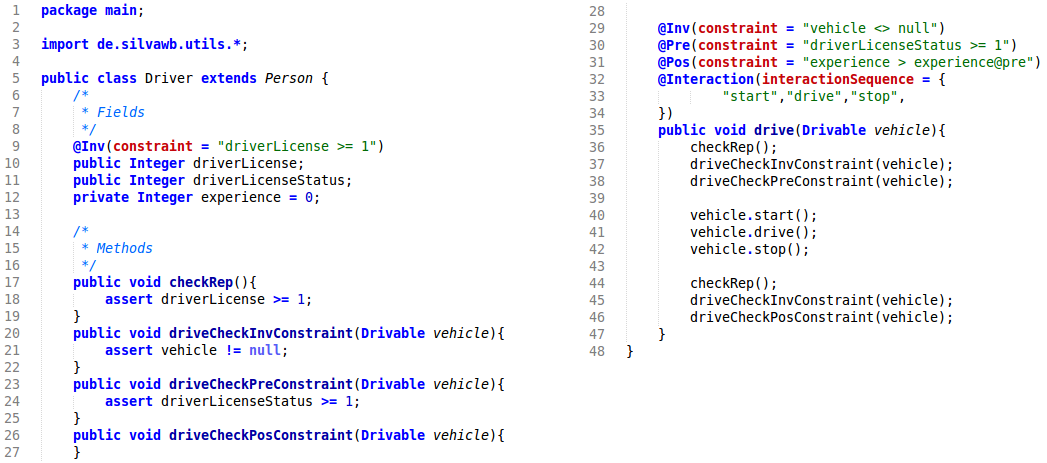
\includegraphics[width=\textwidth]{javaMetamodelExample01_Text}
    \end{center}
    \label{fig:java_metamodel_example_text01}
    \legend{Source: The Author.}
\end{figure}

%---------------------------------------------
% Section
%---------------------------------------------
\section{Relations}
%TODO: First person
With all the meta-models defined, the definition of the relations between their elements can be done. In order to accomplish that, TGG is used to code the relations, because it has been extensively used in current academic research; and is supported by several tools for synchronization. Other options included the \emph{ATL} \citep{jouault2008atl}, which does not seem to be enough ripe for our use; or the \emph{Henshin} \citep{arendt2010henshin}, that is not widely supported for the best synchronization tools \citep{hildebrandt2013survey}. A theoretical basis of TGG has been given in the chapter \ref{ch:foundations}. Here the most representative relations are presented as well as some explanations over them.

%TODO: anex the rest as appedix?

%-------------------
% Subsection
%-------------------
\subsection{Relations between \emph{Uml Class Diagram} and \emph{Java}}
\label{subsec:umlClassDiagram2Java}
Fig. \ref{fig:umlClassDiagram2java_type} shows the triple type graph for the relations between the \emph{UmlClassDiagram} (left) and the \emph{Java} (right) domains, with the correspondence domain being in the middle. In this graph, elements from the left domain are connected to the elements on the right domain, with whom they have a relation. So the element \emph{Model} in \emph{UmlClassDiagram} has a relation to the element \emph{System} in \emph{Java}; analogously, a \emph{Property} in \emph{UmlClassDiagram} is related to an \emph{Field} in \emph{Java}, namely whenever the former is created, the correspondent latter has to be created according to the former's characteristics (i.e. name, type, the class it belongs, etc.).

\begin{figure}[H]
    \caption{The triple type graph for \emph{Uml Class Diagram} and \emph{Java}}
    \begin{center}
        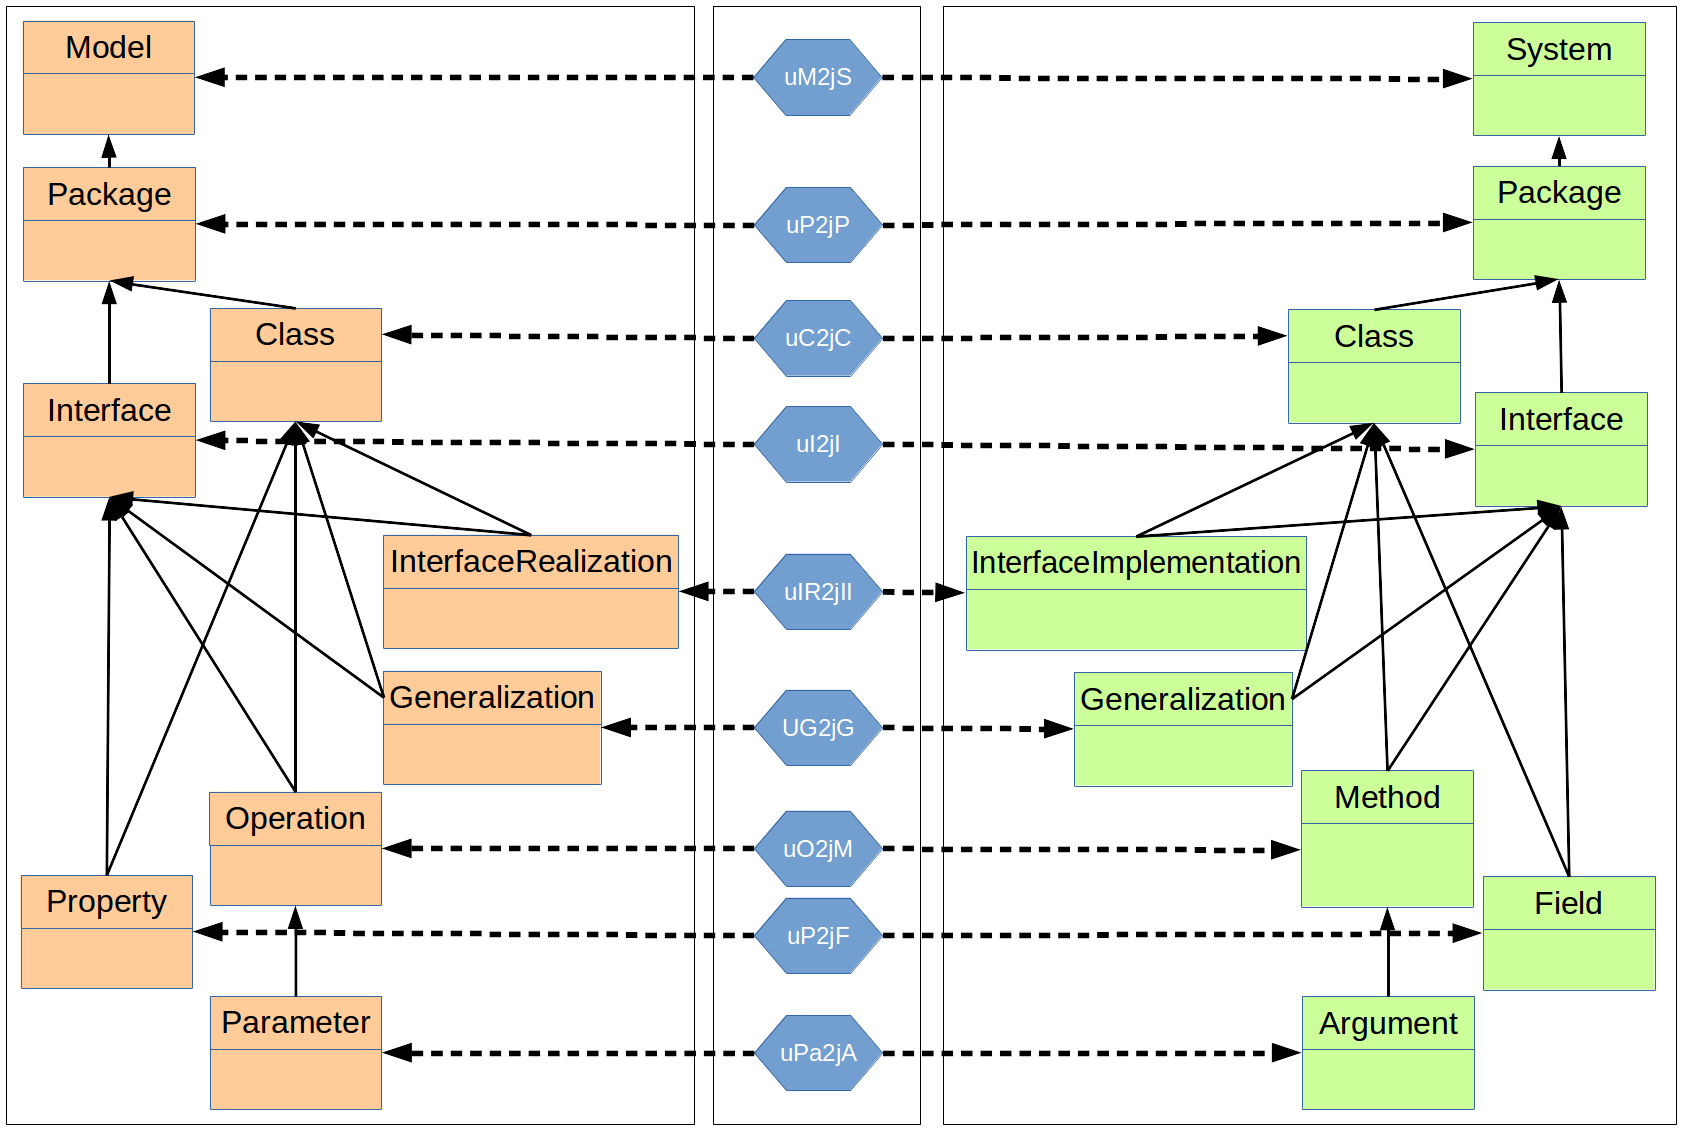
\includegraphics[width=.7\textwidth]{umlClassDiagram2java_type}
    \end{center}
    \label{fig:umlClassDiagram2java_type}
    \legend{Source: The author}
\end{figure}

\begin{figure}[h]
    \caption{The triple rule \emph{uClassAttribute2jClassField}}
    \begin{center}
       	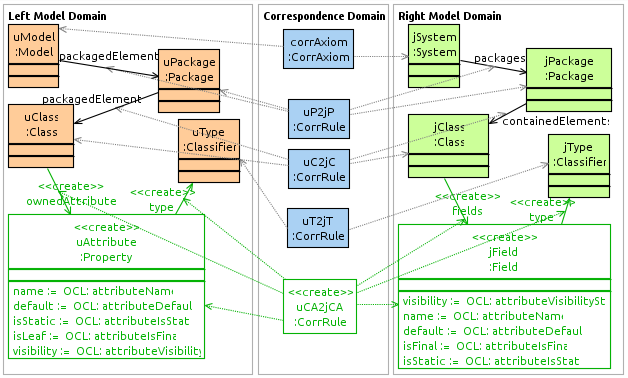
\includegraphics[width=.7\textwidth]{uCAttribute2jCField}
    \end{center}
    \label{fig:uCAttribute2jCField}
    \legend{Source: Image created by the author using the \emph{Eclipse IDE}.}
\end{figure}

The triple rules describing the relation between \emph{Model} and \emph{System}, as well as \emph{Package}(UML) and \emph{Package}(Java) is available on fig. \ref{fig:tgg_rule}. The triple rule encoding the relation between an \emph{Attribute} of a \emph{Class} in \emph{UmlClassDiagram} and a \emph{Field} of a \emph{Class} in \emph{Java} is shown on fig. \ref{fig:uCAttribute2jCField}. In essence, this rule formalize the fact that for every \emph{Class Attribute} (white filling in the image) in \emph{UmlClassDiagram} a correspondent \emph{Class Field} in \emph{Java} is supposed to exist with corresponding values for the respective meta-attributes. These are in the \emph{UML Property} \emph{name}, \emph{default}, \emph{isStatic}, \emph{isLeaf}, and \emph{visibility}, which correspond in order to \emph{name}, \emph{default}, \emph{isStatic}, \emph{isFinal}, and \emph{visibility} in the \emph{Java Field}.

\begin{figure}[h]
    \caption{The triple rule \emph{uInterfaceRealization2jInterfaceImplementation}}
    \begin{center}
       	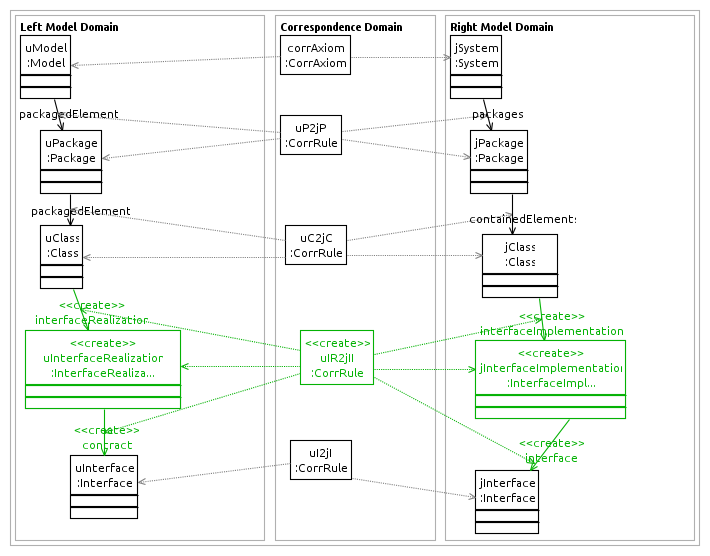
\includegraphics[width=.7\textwidth]{uIRealization2jIImplementation}
    \end{center}
    \label{fig:uIRealization2jIImplementation}
    \legend{Source: Image created by the author using the \emph{Eclipse IDE}.}
\end{figure}

Analogously, the figure \ref{fig:uIRealization2jIImplementation} shows the triple rule $L_sL_cL_t \rightarrow R_sR_cR_t$ for \emph{UML InterfaceRealization} and \emph{Java InterfaceImplementation}. In this case, an \emph{InterfaceRealizations} have none meta-attributes to be described, besides the associations with \emph{Class} and \emph{Interface}. This rule could be as as follows: Given a state $S_i$ with a triple graph $L_sL_cL_t$ (LHS) containing all the color-filled in fig. \ref{fig:uIRealization2jIImplementation}, the creation of a \emph{UML InterfaceRealization} ($uInterfaceRealization \in R_s$) implies the creation of a \emph{Java InterfaceImplementation} ($uInterfaceImplementation \in R_t$) connected by an element of the correspondence domain ($uIR2jII \in R_c$) and vice-versa. The problem with this transformation is that it does not encode the fact that the implementing class in Java (\emph{jClass}) should contain the $m$ methods defined by the interface (\emph{uInterface}). A possible solution would be the creation of a new rule including an object (\emph{uMethod}) contained by (\emph{uInterface}) in $L_s$ linked with the respective \emph{jMethod} contained in \emph{jClass} in $R_t$ (RHS). This new rule should then be evaluated $m$ times by the transformation engine (for the creation of the $m$ methods in \emph{jClass}), but in fact it can be executed only once in the operational semantic scheme proposed by \citet[p. 9]{giese2010toward}. In the same scheme, the creation of such rule would entail a critical pair, given that two different rules have the object \emph{uInterfaceRealization} in the $R_s$. A definite solution is not know by us, therefore this synchronization task ends up being left to the developer.

\begin{figure}[h]
    \caption{Example of forward synchronization from a \emph{UMLClassDiagram} model (left) and a \emph{Java} (right) model}
    \begin{center}
       	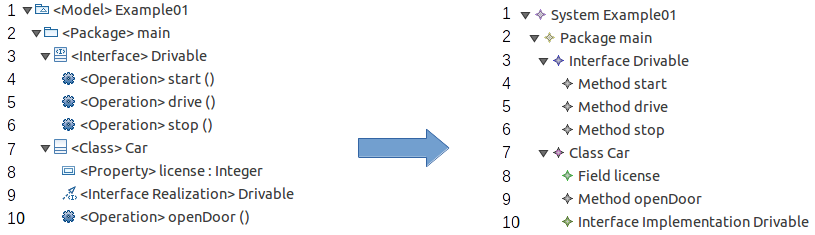
\includegraphics[width=.9\textwidth]{umlClassDiagram2java_Example01}
    \end{center}
    \label{fig:umlClassDiagram2java_Example01}
    \legend{Source: Image created by the author using the \emph{Eclipse IDE}.}
\end{figure}


Fig. \ref{fig:umlClassDiagram2java_Example01} shows the result of a forward transformation from \emph{UMLClassDiagram} to \emph{Java} executed by the \emph{MoTE transformation tool} based on the rules presented in this section plus some simpler rules not shown here (i.e \emph{uModel2jSystem}, \emph{uPackage2jPackage}, \emph{uClass2jClass}, emph{uCOperation2jCOperation} and \emph{uIOperation2jIOperation}).

%-------------------
% Subsection
%-------------------
\subsection{UmlInteraction2Java}
\label{subsec:UmlSequenceDiagram2Java}
FIGURE \ref{fig:uILifeline2jMAnnotation} to \ref{fig:uMessageSequence2jInteractionAnnotation_2}

\begin{figure}[h]
    \caption{}
    \begin{center}
        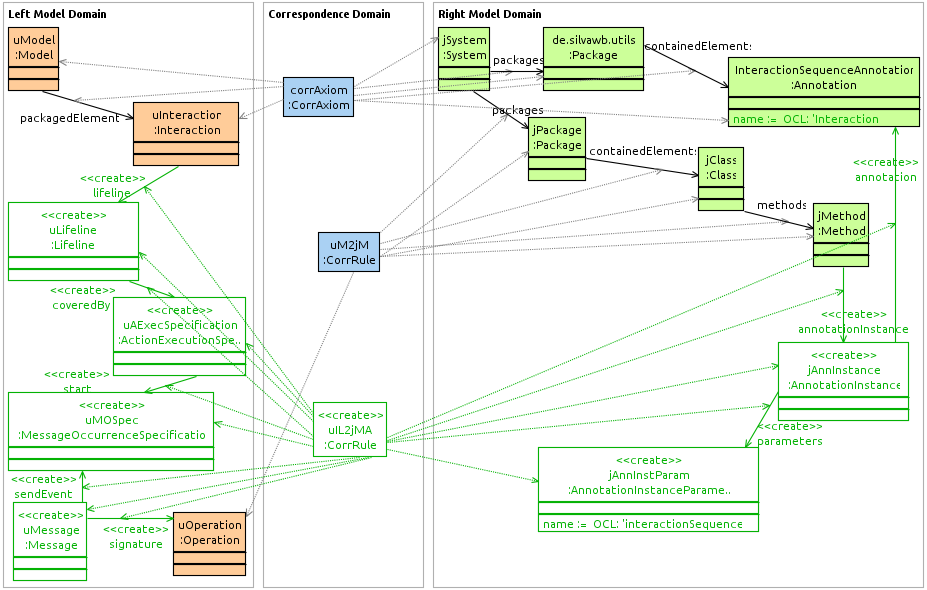
\includegraphics[width=40em]{uILifeline2jMAnnotation}
    \end{center}
    \label{fig:uILifeline2jMAnnotation}
    \legend{Source: Image created by the author using the \emph{Eclipse IDE}.}
\end{figure}
\begin{figure}[h]
    \caption{}
    \begin{center}
        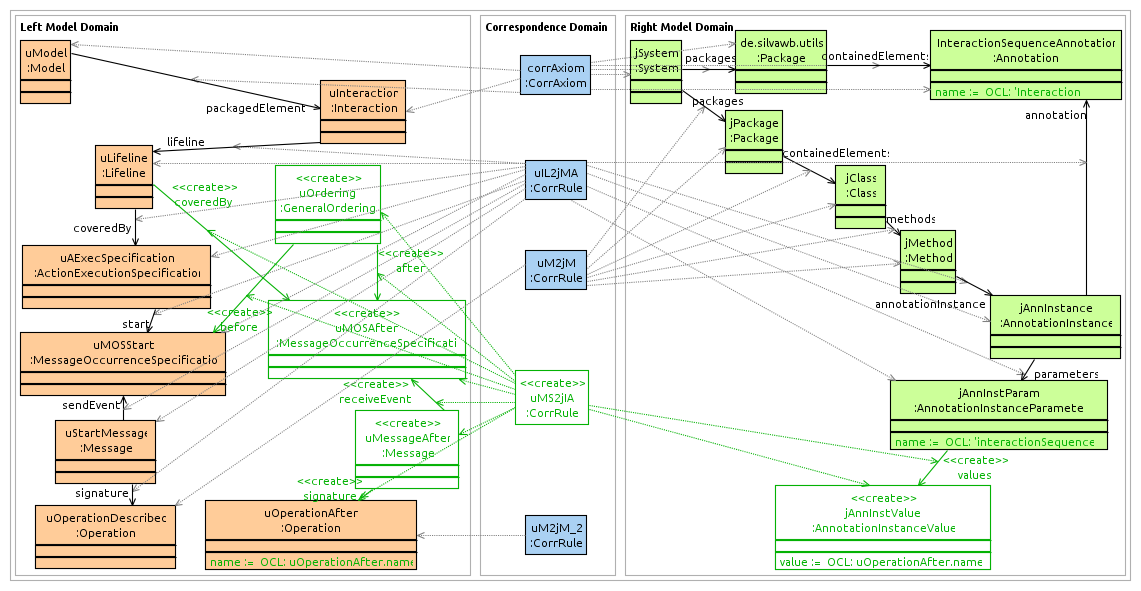
\includegraphics[width=40em]{uMessageSequence2jInteractionAnnotation}
    \end{center}
    \label{fig:uMessageSequence2jInteractionAnnotation}
    \legend{Source: Image created by the author using the \emph{Eclipse IDE}.}
\end{figure}
\begin{figure}[h]
    \caption{}
    \begin{center}
        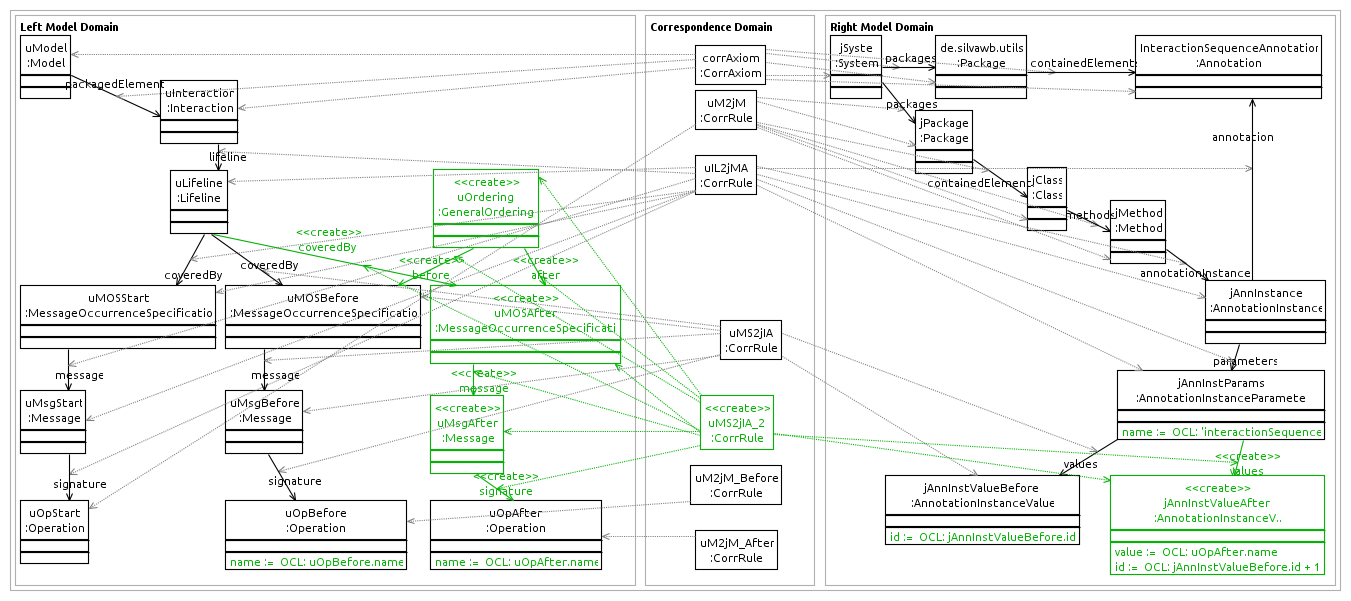
\includegraphics[width=40em]{uMessageSequence2jInteractionAnnotation_2}
    \end{center}
    \label{fig:uMessageSequence2jInteractionAnnotation_2}
    \legend{Source: Image created by the author using the \emph{Eclipse IDE}.}
\end{figure}


%-------------------
% Subsection
%-------------------
\subsection{UmlContracts2Java}
\label{subsec:UmlContracts2Java}
FIGURE \ref{fig:uCInv2jCInv} to \ref{fig:uOPPreInt2jMAPreAssert}

\begin{figure}[h]
    \caption{}
    \begin{center}
        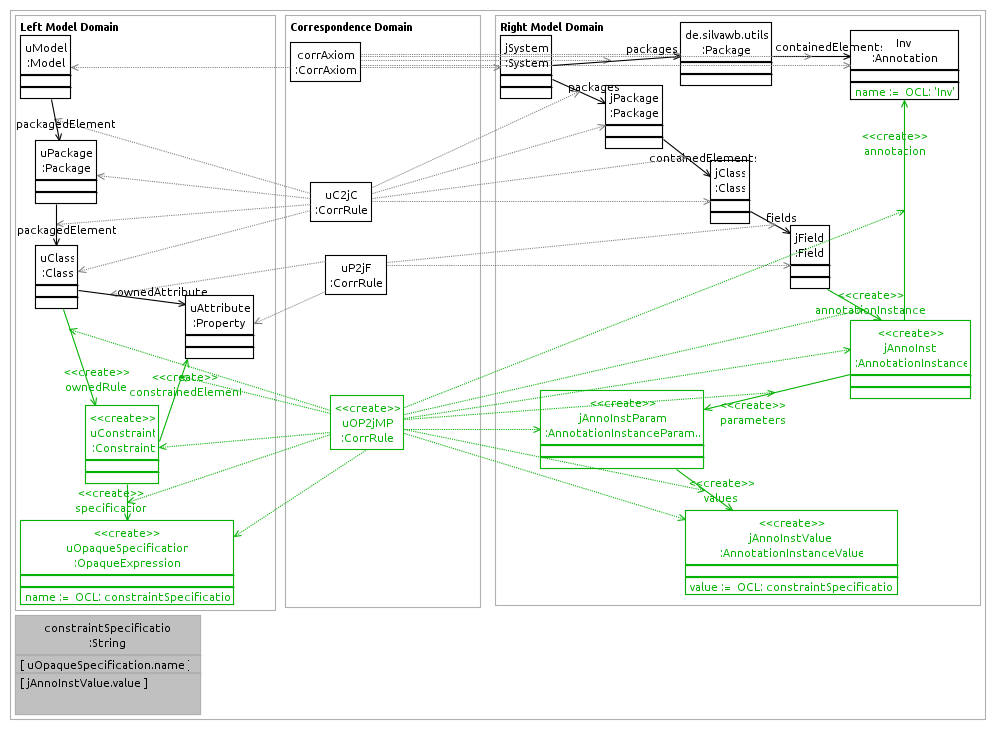
\includegraphics[width=40em]{uCInv2jCInv}
    \end{center}
    \label{fig:uCInv2jCInv}
    \legend{Source: Image created by the author using the \emph{Eclipse IDE}.}
\end{figure}
\begin{figure}[h]
    \caption{}
    \begin{center}
        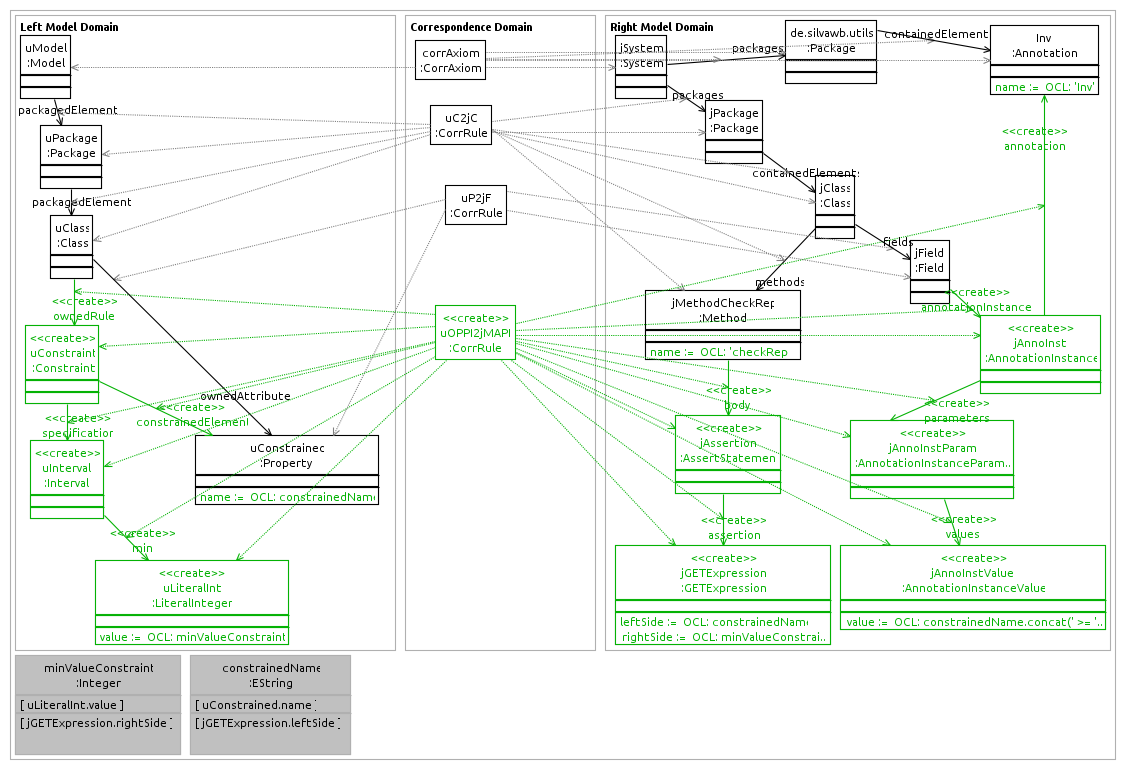
\includegraphics[width=40em]{uCInvInt2jCInvAssert}
    \end{center}
    \label{fig:uCInvInt2jCInvAssert}
    \legend{Source: Image created by the author using the \emph{Eclipse IDE}.}
\end{figure}
\begin{figure}[h]
    \caption{}
    \begin{center}
        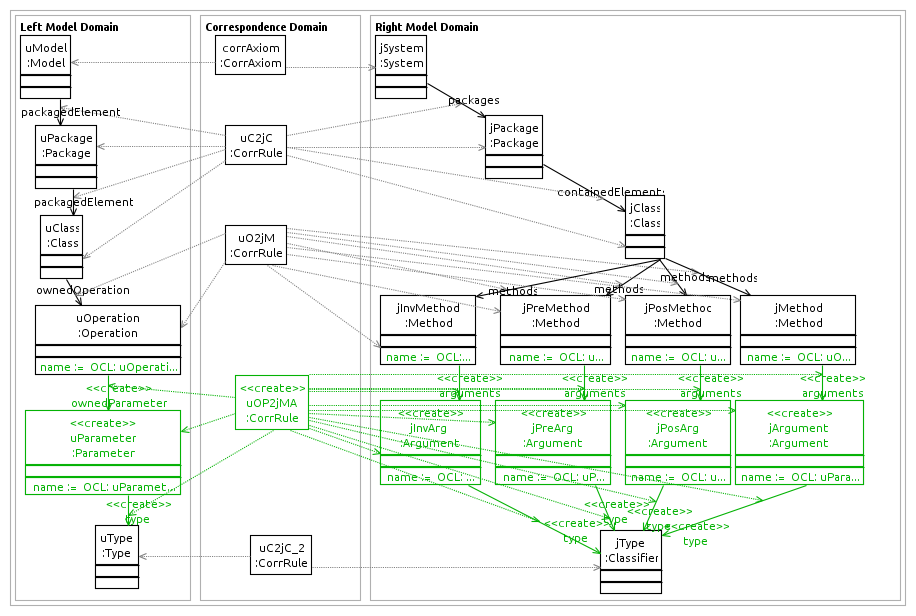
\includegraphics[width=40em]{uOParamenter2jMArgument}
    \end{center}
    \label{fig:uOParamenter2jMArgument}
    \legend{Source: Image created by the author using the \emph{Eclipse IDE}.}
\end{figure}
\begin{figure}[h]
    \caption{}
    \begin{center}
        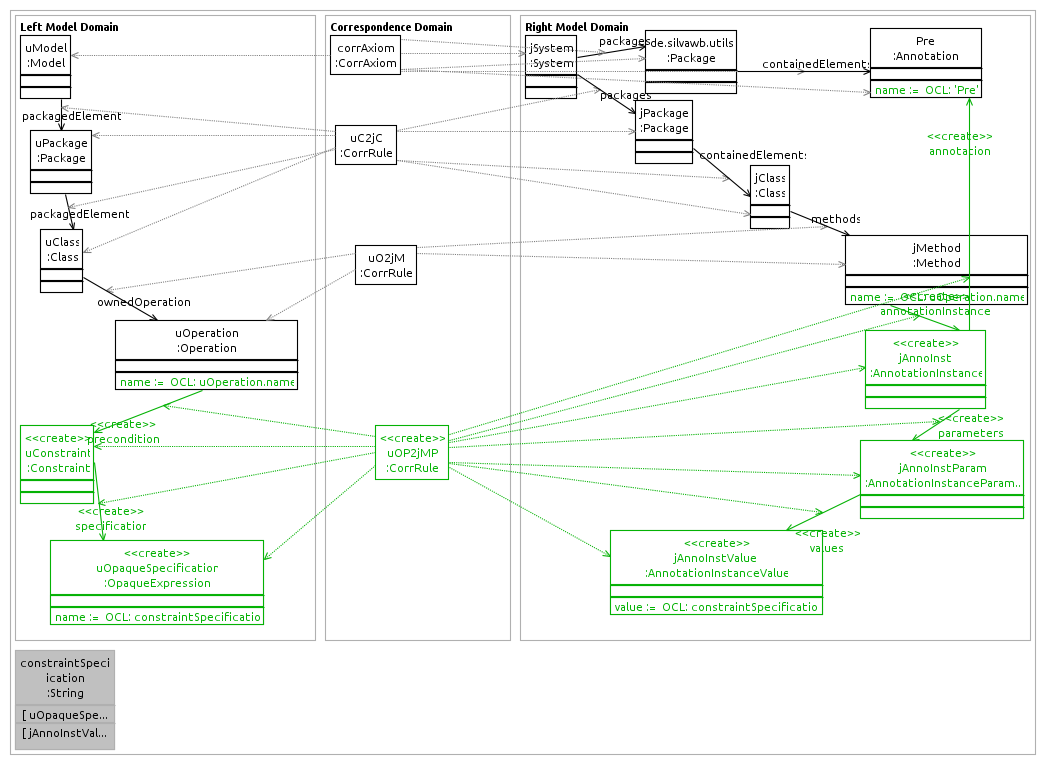
\includegraphics[width=40em]{uOPPre2jMAPre}
    \end{center}
    \label{fig:uOPPre2jMAPre}
    \legend{Source: Image created by the author using the \emph{Eclipse IDE}.}
\end{figure}
\begin{figure}[h]
    \caption{}
    \begin{center}
        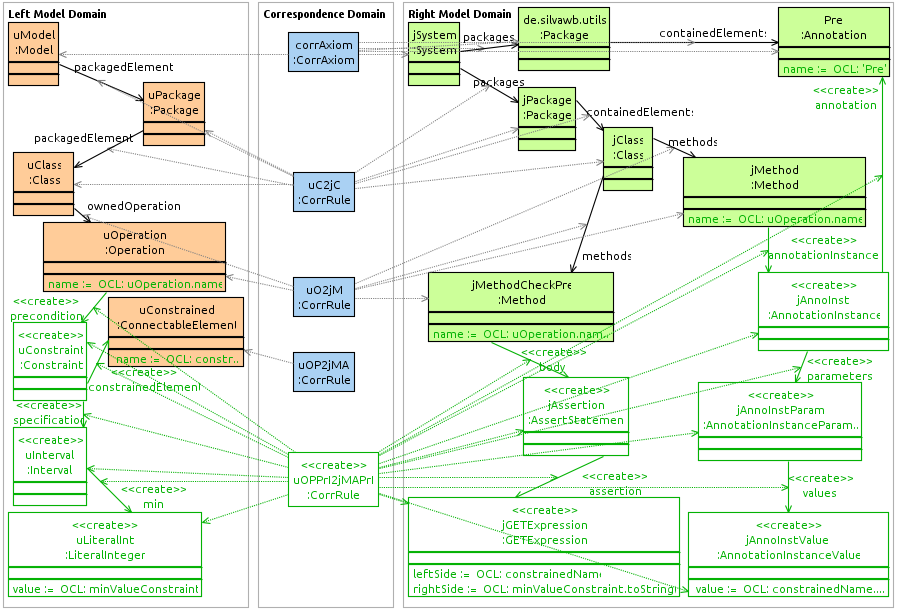
\includegraphics[width=40em]{uOPPreInt2jMAPreAssert}
    \end{center}
    \label{fig:uOPPreInt2jMAPreAssert}
    \legend{Source: Image created by the author using the \emph{Eclipse IDE}.}
\end{figure}

%%%%%%%%%%%%%%%%%%%%%%%%%%%%%%%%%%%%%%%%%%%%%%%%%%%%%%%%%%%%%%%%%%%%%%%%
% Chapter
%%%%%%%%%%%%%%%%%%%%%%%%%%%%%%%%%%%%%%%%%%%%%%%%%%%%%%%%%%%%%%%%%%%%%%%%
\chapter{Synchronization of Models in the Java Technological Space}
\label{chapter:metamodel_synchronization}

%TODO: Update subsections if necessary
In the last chapter the relations between some meta-models of the Java technological space were presented in terms of triple graphs, organized as triple rules and consequently in triple graph grammars. Each TGG was shown in a different subsection (namely \ref{subsec:umlClassDiagram2Java}, \ref{subsec:UmlSequenceDiagram2Java} and \ref{subsec:UmlContracts2Java}) and represents a different edge of the network of models built (see fig. \ref{fig:network_metamodels}). By being so, each edge corresponds to a different synchronization problem and can be sold, generally speaking, independently from the others. most of the research in the realm deals with such situation. Therefore there are several approaches attempting to solve model synchronization between two models using TGG.

Between them is the \emph{FUJABA} \citep{nickel2000fujaba}, a standalone application that uses TGG to code the relations. Or the \emph{CoWolf}, an extensible framework based on \emph{Eclipse Plug-ins} supporting a pair of meta-models according to \citet{getircowolf}, but that uses \emph{Henshin} \citep{arendt2010henshin} to encode the relations. Finally there is the \emph{MoTE} transformation tool, a series of \emph{Eclipse Plug-ins} for creating TGG's, both graphically and textually; and for transforming models based on these TGG's. We take \emph{MoTE} for the most adequate option for our needs, mainly because of extensive literature about it (\citep{giese2009efficient} and \citep{hildebrandt2012mdelab}) and the easy integration with other technologies, like the \emph{EMF Ecore} or other useful \emph{Eclipse Plug-ins}.

\begin{figure}[h]
    \caption{Synchronization scheme of the \emph{MoTE} tool}
    \begin{center}
        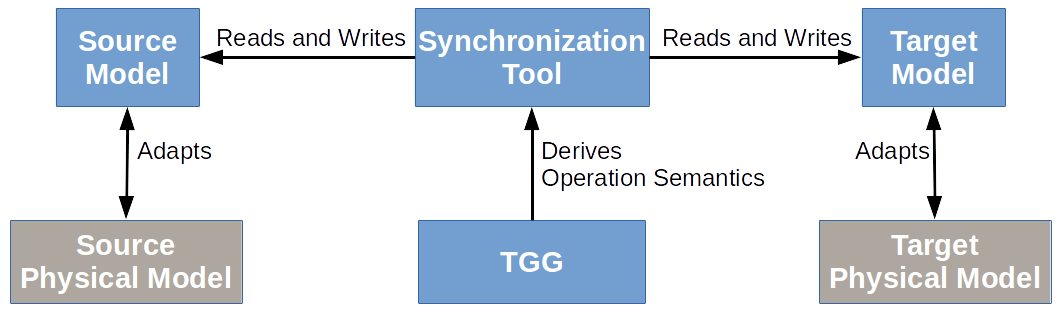
\includegraphics[width=25em]{MoTE_scheme}
    \end{center}
    \label{fig:MoTE_scheme}
    \legend{Source: Adapted from \citep{giese2010model}.}
\end{figure}

The figure \ref{fig:MoTE_scheme} summarizes how the \emph{MoTE} tool works. Basically, the input TGG is used to derive the operational semantics of the transformation between the source and target models, which are read and written by the synchronization tool. Only these first components (highlighted in the picture) are treated in this thesis. Note, however, that the final practical application of the synchronization is only possible through the adaptation of the logical models (presented so far in form of abstract syntax, e.g \ref{fig:java_metamodel_example}) to physical models (presented so far in form of concrete syntax, e.g \ref{fig:java_metamodel_example_text01}).

As stated before, there exists one synchronization scheme similar to fig. \ref{fig:MoTE_scheme} for each edge of our network of models. But as the whole network have to be maintained, it raises the problem of synchronizing not only two models separately, but instead a whole set of models. In this scenario, each modification on a specific model has to be propagated through the net. For that, a theoretical analysis of the problem, followed by an algorithm is presented below.

%---------------------------------------------
% Section
%---------------------------------------------
\section{Synchronizing the Network of Models}
As stated in the chapter \ref{ch:foundations}, a \emph{network of models} is a graph $G = (V,E)$, with $V$ being the models and $E$ the edges linking each pair of related models. When one of these vertices $v \in V$ undergoes changes, all its direct neighbors $N(v)$ have to be updated (synchronized) accordingly. As they possibly undergo changes in the process, their neighbors have to be synchronized too, as well as the next neighbors and so on. The preoccupation here is to describe an algorithm to propagate such modifications, and analyze some properties of this algorithm.

A synchronization is then defined as a function $sync: S \times S \times \Delta_S \times T \rightarrow T \times \Delta_T$, where $sync (s_0, s_1, \delta_s, t_0) = (t_1, \delta_t)$ means that, given a source model $s_0$ synchronized with the target model $t_0$; a new updated source model $s_1$; and $\delta_s$ representing the modifications over $s_0$ that produced $s_1$; a new model $t_1$ synchronized with $s_1$ is produced together with the modifications $\delta_t$ necessary for such process. Here two important assumptions were made:

\begin{itemize}
\item \textbf{Supposition 1:} Only one model can be modified at a time, this means only one vertex can be modified at a time in the whole network $-$ two models are not allowed to be modified simultaneously. This does not seems to be a very problematic restriction, once that in a practical scenario the models could be maintained centralized and observed for changes. Whenever it happens, the synchronization algorithm is ran. 

\item \textbf{Supposition 2:} A synchronization execution has a direction: Whether forward or backward, but not both at the same time. In the first case the source model (that underwent user changes) updates the target model, but does not have side effects, meaning that the synchronization does not provoke extra modification besides the user's ones. To put in other words, in one step the synchronization effects does not ripple back to the source, instead it goes only further.

\item \textbf{Corollary 1:} One single execution of $sync (s_0, s_1, \delta_s, t_0)$ is enough to synchronize $s_1$ with $t_0$.
\end{itemize}

The goal of this paper is not the definition of the $sync$ algorithm, but the definition of an algorithm for the synchronization of a whole network of models.

This synchronization is performed through a function $netsync: (V,E) \times V \times V \times \Delta_S \rightarrow (V,E)$, where $netsync ((V_0,E_0), s_0, s_1, \delta_s) = (V_1,E_1)$ means that for the synchronized network $(V_0,E_0)$ containing the vertex $s_0 \in V_0$, whose model underwent $\delta_s$ modifications, resulting in $s_1$, a new network of synchronized models $(V_1,E_1)$ is delivered. The $netsync$ algorithm is defined in the listing \ref{lst:NetSync}.

%Algorithm
\lstinputlisting[label=lst:NetSync, caption=neysync imperative algorithm definition]{algorithm/netsync_00.alg}

Firstly the initial network is updated with the new vertex $s1$, then every neighbor $ni$ of $s$ is synchronized according to the modifications $ds$. If it causes modifications on $ni$, then the network is recursively further synchronized starting from $ni$. Extra assumptions were made by this algorithm:

\begin{itemize}
\item \textbf{Supposition 3:} The input network of models $(V0,E0)$ is finite.

\item \textbf{Supposition 4:} The input network of models $(V0,E0)$ has no cycles.
\end{itemize}

This implies the following properties:

\begin{itemize}
\item \textbf{Theorem 1:} The algorithm always terminates. Because supposition 2 is made, it suffices only one call to $sinc$ on line 4, representing the synchronization of $s0$ and $ni$ $-$ i.e the edge $(s0,ni)$), to synchronize both models (see corollary 1). Furthermore, every edge synchronization is followed by maximal one recursive call on line 8. As the set of edges is finite (Supposition 3), so is the amount of recursive calls (line 8) and so is the number of loops iterating over any vertex neighbors (lines 3 to 10). So is guaranteed the termination of the algorithm.

\item \textbf{Theorem 2:} The time complexity of $netsync((V0,E0), s0, s1, ds)$ is in the worst case $O(\Delta(V0,E0) |E0|)$, where a $sync$ call is taken as elementary operation.

\item \textbf{Theorem 3:} The algorithm is deterministic...
\end{itemize}

DISCUSS CYCLE; TGG for Multiple models

%%%%%%%%%%%%%%%%%%%%%%%%%%%%%%%%%%%%%%%%%%%%%%%%%%%%%%%%%%%%%%%%%%%%%%%%
% Chapter
%%%%%%%%%%%%%%%%%%%%%%%%%%%%%%%%%%%%%%%%%%%%%%%%%%%%%%%%%%%%%%%%%%%%%%%%
\chapter{Conclusion and Discussion}
%TODO: Synchronization was showcased?
%TODO: Other meta-model developed?
%TODO: umlClass2java is the name?
A network of meta-models of the Java technological space was developed, comprising a set of common meta-models used in Java software and the respective relations between them, as well as synchronization between the models was showcased, demonstrating as final result that the construction of such network and the employment of synchronization has worked and moreover seems to be promising. Despite the outcomes are not complete and not ripe enough to be put in practice, the ideas and the insights reported plus the summary of the state-of-art are valuable for current research and thus contributing.

In the first phase some meta-models were developed (e.g Java), and in the second phase the relations were coded (e.g. umlClass2java). In regard to these both steps the main legacy are the novel relations between some elements of some meta-models (e.g. the relation between UML contracts and Java assertions). The third phase serve to demonstrate briefly the application of synchronization in the practice. Most of the initially set up goals were achieved, even though the relations could rather be more extensive, likewise a more comprehensive synchronization demonstration would be desired.

%TODO: Talk more? Summarize all?

%TODO: How should I cite Oracle
Some difficulties were found along the work, but they absolutely did not obstructed the success of the final result. The first one the lack of openly available meta-models in the literature or by the vendors. For instance \emph{Oracle} does not publicize any standard meta-model for Java, nor are them easily to find in the literature. One may find alternative versions in the source code of IDE's, but it still requires some cost. Moreover, they are sometimes because their format incompatible with the employed tool, what also hinders the progress of someone's work. The result of this thesis may be a partial solution for that, although meta-models of other technological spaces still lack a similar work. Another complication are the lack of documentation of some tools $-$ in special the \emph{MoTE} $-$, that makes both the flow of the development and eventual debug tasks sometimes troublesome. \emph{MoTE} might have publications about it and also a good reputation in the community, but a extensive broad documentation of the plug-in for the \emph{Eclipse IDE} is needed. At last, but not least is the performance problem of such tools. Both the \emph{EMF} and \emph{MoTE} need to generate Java code in order to run the synchronization procedure, and with big models this process happens to cost a considerable computation time.

Some points become therefore remarkable for future work. Firstly, an easy to find and accessible tutorial or instructions for the theoretic and practical basis of triple graph grammars is valuable in order to make the use of models synchronization popular among engineers or software developers, who sometimes are not very used to the area and thus express a big rejection to apply such technique in their projects.

Secondly, the work of this thesis can be naturally continued and expanded, by completing the identification of relation between the meta-model or by creating meta-models that satisfy completeness. Not to mention, such relations could be expressed in other languages (e.g. \emph{ATL}) and the same work extended to other technological spaces (e.g. COBOL, C\#).

Furthermore, the implementation of a \emph{Eclipse} plug-in should not be a big problem, since the \emph{MoTE} already generates a plug-in for the execution of its algorithm. So the task in this case would be enhance it with a user-friendly interface plus new functionalities and naturally a slightly more practical approach (e.g. handling of actual Java code instead of quasi-theoretic scenarios like Java expressed in XML files).

And lately, a relatively big issue is the use of TGG's for non-MOF-compliant meta-models $-$ or meta-models that are not naturally seen as MOF-compliant, e.g. the complete Java model. Because under certain conditions it could be interesting to see such models from another point of view than the MOF. A clear example is source-code, which can be treated in an easier way with abstract syntax trees. \citet{angyal2008novel} suggests a method to treat this case, but anyways it still remains an open problem and certainly a future challenge.

%TODO: Problem on interface several methods

%TODO: Include this? no study known by us presents an effective tool, that could be used extensively in practice. We believe though, that the contribution of this thesis can be useful for the creation of such a tool.

%TODO: Include this? It means, that the success of this thesis brings the contribution towards the definition of a network of interconnected meta-models useful to both research and industry community. Therefore the availability of such a network might finally allow the extensive use of Model-driven Engineering in practice $-$ helping bridging the gap between system abstractions and their concrete form $-$ and foster the further development of more sophisticated model synchronization methods.

%TODO: enhance the network presented on section 4.1

%TODO: Enhance algortihm network sync + theoretical basis

%%%%%%%%%%%%%%%%%%%%%%%%%%%%%%%%%%%%%%%%%%%%%%%%%%%%%%%%%%%%%%%%%%%%%%%%
% Bibliography
%%%%%%%%%%%%%%%%%%%%%%%%%%%%%%%%%%%%%%%%%%%%%%%%%%%%%%%%%%%%%%%%%%%%%%%%
%TODO: Adjust to UFRGS style? see iiufrgs
\bibliographystyle{plainnat}
\bibliography{biblio}

\end{document}